\documentclass[12pt]{report}
\usepackage[utf8]{inputenc}
\DeclareUnicodeCharacter{03B8}{$\theta$}
\DeclareUnicodeCharacter{03C6}{$\phi$}
\DeclareUnicodeCharacter{03A9}{$\Omega$}
\DeclareUnicodeCharacter{03C9}{$\omega$}
\usepackage{amsmath, amssymb} 
\usepackage{graphicx} 
\usepackage{float}
\usepackage{svg} % <--- Added to allow SVG insertion
\svgsetup{inkscapelatex=false}
\usepackage{mathptmx} % Changes the font to Times New Roman
\usepackage{setspace}
\usepackage{ragged2e}
\setstretch{2.2}
\raggedbottom
\setlength{\textfloatsep}{10pt plus 2pt minus 2pt}
\setlength{\floatsep}{8pt plus 2pt minus 2pt}
\setlength{\intextsep}{8pt plus 2pt minus 2pt}
\pdfsuppresswarningpagegroup=1

% --- THE MARGIN FIX FOR BOOKBINDING ---
% Added 'footskip=0.5in' to pull the page number up, and increased bottom margin
\usepackage[paperwidth=21cm, paperheight=29cm, left=1.5in, right=1in, top=1.2in, bottom=1.5in, footskip=0.5in]{geometry}

% --- The Double-Line Page Border Setup ---
\usepackage{tikz}
\usetikzlibrary{decorations.text,decorations.pathmorphing}
\usepackage{eso-pic}
\usepackage{xcolor}
\definecolor{defaultbordercolor}{HTML}{000000}
\newcommand{\setbordercolorforpage}[2]{\expandafter\gdef\csname bordercolor@#1\endcsname{#2}}
\newcommand{\resolvebordercolor}[1]{%
  \ifcsname bordercolor@#1\endcsname
    \colorlet{currentbordercolor}{\csname bordercolor@#1\endcsname}%
  \else
    \colorlet{currentbordercolor}{defaultbordercolor}%
  \fi
}
% Example usage: \setbordercolorforpage{12}{red}
\AddToShipoutPictureBG{%
  \begin{tikzpicture}[remember picture, overlay]
    \resolvebordercolor{\number\value{page}}
    % Lowered the yshift from 0.8in to 0.4in to push the bottom border down
    \draw[color=currentbordercolor, line width=1pt, double, double distance=2pt]
         ([xshift=1.2in, yshift=0.4in]current page.south west) rectangle
         ([xshift=-0.8in, yshift=-0.8in]current page.north east);
  \end{tikzpicture}
}

% --- Removes chapter numbers from chapters like Certificate/Acknowledgement ---
\usepackage{titlesec}
\usepackage{microtype}
\usepackage{hyperref}
\usepackage{needspace}
\usepackage{etoolbox}
\definecolor{chapterstrawberry}{HTML}{FC4C4E}
\definecolor{sectionnavy}{HTML}{0A1172}
\definecolor{frontmatterolive}{HTML}{0D3E43}
\definecolor{sectionheadingnavy}{HTML}{0A1172}
\definecolor{subsectionheadingrose}{HTML}{C2185B}
\titleformat{\chapter}[display]
  {\normalfont\huge\bfseries\centering\color{chapterstrawberry}}{\chaptername\ \thechapter}{1em}{\Huge}
\titleformat{name=\chapter,numberless}[display]
  {\normalfont\huge\bfseries\centering\color{frontmatterolive}}{}{0pt}{\Huge}
\titleformat{\section}
  {\normalfont\Large\bfseries\color{sectionheadingnavy}}{\thesection}{1em}{}
\titleformat{\subsection}
  {\normalfont\large\bfseries\color{subsectionheadingrose}}{\thesubsection}{1em}{}
\hypersetup{hidelinks}
\pretocmd{\section}{\needspace{5\baselineskip}}{}{}

% --- Reusable metadata ---
\newcommand{\StudentName}{Reet Kumari}
\newcommand{\GuideName}{Dr. ABHISHEK KUMAR}
\newcommand{\DepartmentName}{Department of Physics}
\newcommand{\CollegeName}{J.D. Women's College, Patna}
\newcommand{\UniversityName}{Patliputra University, Patna}
\newcommand{\ClassRollNo}{24}
\newcommand{\ExamRollNo}{2520891050018}
\newcommand{\RegistrationNo}{1920523111050001}
\newcommand{\SessionYears}{2024--2026}
\newcommand{\WhiteCoverXShift}{0pt}
\newcommand{\WhiteCoverYShift}{0pt}
\newcommand{\DeclarationXShift}{0pt}
\newcommand{\DeclarationYShift}{0pt}
\newcommand{\CertificateXShift}{0pt}
\newcommand{\CertificateYShift}{0pt}
\newcommand{\AcknowledgementXShift}{0pt}
\newcommand{\AcknowledgementYShift}{0pt}
\newcommand{\FrontMatterBodyWidth}{0.68\textwidth}
\newcommand{\FrontMatterBodyOffset}{-0.18cm}
\newcommand{\FrontMatterTitleSize}{21}
\newcommand{\FrontMatterTitleLeading}{24}
\newcommand{\FrontMatterBodySize}{15}
\newcommand{\FrontMatterBodyLeading}{19}

% --- Reusable figure-slot macros (drop files into figures/chX/slot_YY.*) ---
\newcommand{\FigureSlotBase}[2]{figures/ch#1/slot_#2}
\newcommand{\FigureSlotMissing}[2]{%
  \fbox{\parbox[c][0.20\textheight][c]{0.82\textwidth}{\centering
  \textbf{Placeholder figure slot}\\[3pt]
  Chapter #1, Slot #2\\[3pt]
  Drop a file as:\\
  \texttt{figures/ch#1/slot\_#2.(png|jpg|jpeg|pdf|svg)}}}%
}
\newcommand{\InsertFigureSlot}[5][0.7\textwidth]{%
  \begin{figure}[H]
    \centering
    \IfFileExists{\FigureSlotBase{#2}{#3}.pdf}{%
      \includegraphics[width=#1]{\FigureSlotBase{#2}{#3}.pdf}%
    }{\IfFileExists{\FigureSlotBase{#2}{#3}.png}{%
      \includegraphics[width=#1]{\FigureSlotBase{#2}{#3}.png}%
    }{\IfFileExists{\FigureSlotBase{#2}{#3}.jpg}{%
      \includegraphics[width=#1]{\FigureSlotBase{#2}{#3}.jpg}%
    }{\IfFileExists{\FigureSlotBase{#2}{#3}.jpeg}{%
      \includegraphics[width=#1]{\FigureSlotBase{#2}{#3}.jpeg}%
    }{\IfFileExists{\FigureSlotBase{#2}{#3}.svg}{%
      \includesvg[width=#1]{\FigureSlotBase{#2}{#3}.svg}%
    }{%
      \FigureSlotMissing{#2}{#3}%
    }}}}}
    \caption{#4}
    \label{#5}
  \end{figure}
}
\newcommand{\ChTwoFigure}[4][0.7\textwidth]{\InsertFigureSlot[#1]{2}{#2}{#3}{#4}}
\newcommand{\ChThreeFigure}[4][0.7\textwidth]{\InsertFigureSlot[#1]{3}{#2}{#3}{#4}}
\newcommand{\ChFourFigure}[4][0.7\textwidth]{\InsertFigureSlot[#1]{4}{#2}{#3}{#4}}
\newcommand{\ChFiveFigure}[4][0.7\textwidth]{\InsertFigureSlot[#1]{5}{#2}{#3}{#4}}

% --- Reusable front-matter border style ---
\newcommand{\FrontBlueBorder}{%
  \draw[line width=10pt,color=blue!65]
    ([xshift=1.24in,yshift=0.42in]current page.south west) rectangle
    ([xshift=-0.84in,yshift=-0.84in]current page.north east);
  \draw[line width=1.4pt,color=blue!25]
    ([xshift=1.36in,yshift=0.54in]current page.south west) rectangle
    ([xshift=-0.96in,yshift=-0.96in]current page.north east);
}
\definecolor{frontmattergold}{HTML}{B08A5A}
\definecolor{frontmattergoldlight}{HTML}{D8C2A0}
\newcommand{\FrontGoldBorder}{%
  \draw[line width=1.1pt,color=frontmattergold]
    ([xshift=1.28in,yshift=0.52in]current page.south west) rectangle
    ([xshift=-0.88in,yshift=-0.88in]current page.north east);
  \draw[line width=0.5pt,color=frontmattergoldlight]
    ([xshift=1.38in,yshift=0.62in]current page.south west) rectangle
    ([xshift=-0.98in,yshift=-0.98in]current page.north east);
}

\begin{document}
\hypersetup{pageanchor=false}
\pagenumbering{arabic}
\setcounter{tocdepth}{1}
\begingroup
\setstretch{1.20}

% ==========================================
% TITLE PAGE 
% ==========================================
\begin{titlepage}
    \pagecolor{white}
    \color{black}
    \thispagestyle{empty}
    \pagecolor{sectionnavy!95!black}
    \color{blue!88!white}
    \begin{tikzpicture}[remember picture,overlay]
      \draw[line width=1.2pt,color=yellow!55!white]
        ([xshift=1.38in,yshift=0.55in]current page.south west) rectangle
        ([xshift=-0.95in,yshift=-0.95in]current page.north east);
      \draw[line width=0.5pt,color=yellow!35!white]
        ([xshift=1.45in,yshift=0.62in]current page.south west) rectangle
        ([xshift=-1.02in,yshift=-1.02in]current page.north east);
    \end{tikzpicture}

    \centering
    \vspace*{0.45cm}
    {\small \textbf{\color{yellow!80!white}PROJECT REPORT}\\}
    \vspace{0.08cm}
    {\small \textbf{\color{yellow!80!white}ON}\\}
    \vspace{0.5cm}
    \begin{tikzpicture}
      \node at (0,0.00) {
\includegraphics[width=0.25\textwidth]{logo-icon.png}};
      \path[decorate,decoration={text along path,text={|\bfseries\fontsize{14}{16}\selectfont\color{yellow!88!white}|PATLIPUTRA UNIVERSITY},text align=center}]
      (-2.55,0.95) arc[start angle=180,end angle=0,radius=2.55];
    \end{tikzpicture}
    \\
    \vspace{0.08cm}
    {\LARGE \textbf{\color{yellow!95!white}ADVANCED QUANTUM MECHANICS}\\}
    \vspace{0.12cm}
  
    {\large \textbf{\color{yellow!88!white}DEPARTMENT OF PHYSICS}\\}
    \vspace{0.10cm}
    {\Large \textbf{\color{yellow!95!white}J.D. WOMEN'S COLLEGE}\\}
    \vspace{0.10cm}
    {\large \textbf{\color{yellow!88!white}PATLIPUTRA UNIVERSITY, PATNA}\\}
    \vspace{0.18cm}
     
\includegraphics[width=0.18\textwidth]{logo.png}\\
    \vspace{0.16cm}
    {\normalsize \textbf{\color{yellow!90!white}BY}\\}
    \vspace{0.10cm}
    {\large \textbf{\color{yellow!96!white}\MakeUppercase{\StudentName}}\\}
    {\normalsize \color{yellow!88!white}EXAM ROLL NO. -- \ExamRollNo\\}
    {\normalsize \color{yellow!88!white}REGISTRATION NO. -- \RegistrationNo\\}
    {\normalsize \color{yellow!88!white}CLASS ROLL NO. -- \ClassRollNo\\}
    {\normalsize \color{yellow!88!white}SESSION -- \SessionYears\\}

    \vfill
    {\normalsize \textit{\color{yellow!82!white}Under the guidance of :-}\\}
    {\large \textbf{\color{yellow!95!white}\GuideName}\\}
    {\normalsize \color{yellow!88!white}\MakeUppercase{\DepartmentName}\\}
    {\normalsize \color{yellow!88!white}\MakeUppercase{\CollegeName}\\}
    \vspace{0.25cm}
\end{titlepage}
\nopagecolor

% ==========================================
% TITLE PAGE (WHITE BACKGROUND COPY)
% ==========================================
\begin{titlepage}
    \pagecolor{white}
    \color{black}
    \thispagestyle{empty}
    \begin{tikzpicture}[remember picture,overlay]
      \draw[line width=1.2pt,color=sectionnavy!70]
        ([xshift=1.38in,yshift=0.55in]current page.south west) rectangle
        ([xshift=-0.95in,yshift=-0.95in]current page.north east);
      \draw[line width=0.5pt,color=sectionnavy!35]
        ([xshift=1.45in,yshift=0.62in]current page.south west) rectangle
        ([xshift=-1.02in,yshift=-1.02in]current page.north east);
    \end{tikzpicture}

    \centering
    \hspace*{\WhiteCoverXShift}% positive moves right, negative moves left
    \vspace*{\WhiteCoverYShift}% positive moves down, negative moves up
    \vspace*{0.90cm}
    \begin{minipage}[t][0.85\textheight][s]{0.68\textwidth}
    \centering
    {\fontsize{11.5}{14}\selectfont \textbf{PROJECT REPORT ON}\\}
    \vspace{0.22cm}
    {\fontsize{19}{23}\selectfont \textbf{Theory of Scattering}\\}
    \vspace{0.14cm}
    {\fontsize{10.5}{13}\selectfont \textit{(Advanced Quantum Mechanics)}\\}
    \vspace{0.42cm}
    {\fontsize{15.5}{19}\selectfont \textbf{DEPARTMENT OF PHYSICS}\\}
    \vspace{0.16cm}
    {\fontsize{17.5}{21}\selectfont \textbf{J.D. WOMEN'S COLLEGE}\\}
    \vspace{0.16cm}
    {\fontsize{14.5}{18}\selectfont \textbf{PATLIPUTRA UNIVERSITY, PATNA}\\}
    \vspace{0.38cm}
    
\includegraphics[width=0.20\textwidth]{logo.png}\\
    \vspace{0.34cm}
    {\fontsize{11.5}{14}\selectfont \textbf{BY}\\}
    \vspace{0.16cm}
    {\fontsize{16}{19.5}\selectfont \textbf{\MakeUppercase{\StudentName}}\\}
    \vspace{0.04cm}
    {\fontsize{11}{13.5}\selectfont EXAM ROLL NO. -- \ExamRollNo\\}
    \vspace{0.04cm}
    {\fontsize{11}{13.5}\selectfont REGISTRATION NO. -- \RegistrationNo\\}
    \vspace{0.04cm}
    {\fontsize{11}{13.5}\selectfont CLASS ROLL NO. -- \ClassRollNo\\}
    \vspace{0.04cm}
    {\fontsize{11}{13.5}\selectfont SESSION -- \SessionYears\\}
    \vfill
    \vspace{0.15cm}
    {\fontsize{11.5}{14}\selectfont \textit{Under the guidance of :-}\\}
    \vspace{0.12cm}
    {\fontsize{15}{18}\selectfont \textbf{\GuideName}\\}
    \vspace{0.06cm}
    {\fontsize{11.5}{14}\selectfont \MakeUppercase{\DepartmentName}\\}
    {\fontsize{11.5}{14}\selectfont \MakeUppercase{\CollegeName}\\}
    \end{minipage}
\end{titlepage}
\nopagecolor

% ==========================================
% INSERTED ATTACHED PAGE
% ==========================================
\begin{titlepage}
    \pagecolor{white}
    \color{black}
    \thispagestyle{empty}
    \begin{tikzpicture}[remember picture,overlay]
      \FrontGoldBorder
      \node[anchor=north,text=chapterstrawberry,font=\bfseries\fontsize{20}{24}\selectfont]
      at ([yshift=-1.0in]current page.north) {PROJECT REPORT 2026};
    \end{tikzpicture}

    \centering
    \vspace*{1.9cm}

    \begin{tikzpicture}
      \node[opacity=0.12] at (0,0.05) {
\includegraphics[width=0.60\textwidth]{logo-icon.png}};
      \node at (0,1.95) {
\includegraphics[width=4cm]{logo-icon.png}};
      \path[decorate,decoration={text along path,text={|\bfseries\fontsize{25}{27}\selectfont\color{sectionnavy}|PATLIPUTRA UNIVERSITY},text align=center}]
      (-4.95,0.48) arc[start angle=180,end angle=0,radius=4.95];
    \end{tikzpicture}

    \vspace{-0.45cm}
    {\Large \textbf{\color{chapterstrawberry}"THEORY OF SCATTERING"}\\}
    {\large \textbf{\color{sectionnavy}(ADVANCED QUANTUM MECHANICS)}\\}
    \vspace{0.27cm}

    {\Large \textbf{\color{sectionnavy}Submitted to}\\}
    {\Large \textbf{\color{chapterstrawberry}J.D. WOMEN'S COLLEGE, PATNA}\\}
    {\Large \textbf{DEPARTMENT OF PHYSICS}\\}
    {\Large \textbf{SESSION 2024--2026}\\}

    \begin{tikzpicture}[remember picture,overlay]
      \fill[blue!10,opacity=0.65]
      ([xshift=1.28in,yshift=1.15in]current page.south west)
      rectangle
      ([xshift=-0.88in,yshift=2.95in]current page.south east);

      \node[anchor=north west,align=left,text width=2.9in]
      at ([xshift=1.36in,yshift=2.83in]current page.south west) {
      {\large \textbf{\color{chapterstrawberry}NAME OF THE GUIDE}}\\[1.5pt]
      {\large \textbf{\GuideName}\\}
      {\normalsize (HOD), Physics Department\\}
      {\normalsize J.D. WOMEN'S COLLEGE\\}
      {\normalsize PATNA}
      };

      \node[anchor=north west,align=left,text width=2.65in]
      at ([xshift=4.42in,yshift=2.83in]current page.south west) {
      {\large \textbf{\color{chapterstrawberry}SUBMITTED BY}}\\[1.5pt]
      {\large \textbf{\MakeUppercase{\StudentName}}\\}
      {\normalsize Exam Roll No. -- \ExamRollNo\\}
      {\normalsize Reg. No. -- \RegistrationNo\\}
      {\normalsize M.Sc. Physics, IV Semester}
      };
    \end{tikzpicture}
\end{titlepage}

% ==========================================
% DECLARATION PAGE
% ==========================================
\begin{titlepage}
    \pagecolor{white}
    \color{black}
    \thispagestyle{empty}
    \centering
    \begin{tikzpicture}[remember picture,overlay]
      \FrontGoldBorder
    \end{tikzpicture}

    \hspace*{\DeclarationXShift}% positive moves right, negative moves left
    \vspace*{\DeclarationYShift}% positive moves down, negative moves up
    \vspace*{1.95cm}
    {\color{chapterstrawberry}\bfseries\fontsize{\FrontMatterTitleSize}{\FrontMatterTitleLeading}\selectfont DECLARATION\par}
    \vspace{0.75cm}
    \hspace*{\FrontMatterBodyOffset}
    \begin{minipage}{0.60\textwidth}
    \setstretch{1.20}
    \fontsize{\FrontMatterBodySize}{\FrontMatterBodyLeading}\selectfont
    \justifying
    I \textbf{\StudentName} here by declare that this dissertation entitled \textbf{"ADVANCED QUANTUM MECHANICS"} is outcome of my own study taken under the guidance of \textbf{\GuideName\ (HOD)} \DepartmentName, J.D. Women's College Patna. I have duly acknowledged all the source used by me in the preparation of the dissertation.
    \end{minipage}

    \vspace{1.85cm}
    \hspace*{\FrontMatterBodyOffset}
    \begin{minipage}{0.60\textwidth}
    \raggedleft
    {\normalsize \textit{\StudentName}}
    \end{minipage}
\end{titlepage}

% ==========================================
% CERTIFICATE PAGE
% ==========================================
\begin{titlepage}
    \pagecolor{white}
    \color{black}
    \thispagestyle{empty}
    \begin{tikzpicture}[remember picture,overlay]
      \FrontGoldBorder
      \node[anchor=north west,text=frontmattergold,font=\bfseries\fontsize{10.5}{10}\selectfont]
      at ([xshift=1.48in,yshift=-1.02in]current page.north west) {P.G DEPARTMENT OF PHYSICS};
      \node[anchor=north west,text=frontmattergold,font=\bfseries\fontsize{9.5}{9.5}\selectfont]
      at ([xshift=1.48in,yshift=-1.24in]current page.north west) {J.D. Women's College Patna};
      \node[anchor=north east,text=frontmattergold,font=\bfseries\fontsize{10.5}{9.5}\selectfont]
      at ([xshift=-1.15in,yshift=-1.02in]current page.north east) {DATE:- \today};
      
    \end{tikzpicture}

    \centering
    \hspace*{\CertificateXShift}% positive moves right, negative moves left
    \vspace*{\CertificateYShift}% positive moves down, negative moves up
    \vspace*{1.95cm}
    {\color{frontmattergold}\bfseries\fontsize{\FrontMatterTitleSize}{\FrontMatterTitleLeading}\selectfont CERTIFICATE\par}
    \vspace{0.32cm}
    \hspace*{\FrontMatterBodyOffset}
    \begin{minipage}{0.60\textwidth}
    \setstretch{1.05}
    \fontsize{\FrontMatterBodySize}{\FrontMatterBodyLeading}\selectfont
    \justifying
    This is certifying that the dissertation entitled \textbf{"ADVANCED QUANTUM MECHANICS"} is the recorded of the original work done by \StudentName\ M.SC SEM 4th under my supervision. The contents of the research presented in the dissertation have not previously formed the basis award of any degree,certificate of university.
    \end{minipage}

    \vspace{2.05cm}
    \hspace*{\FrontMatterBodyOffset}
    \begin{minipage}{0.60\textwidth}
    \raggedleft
    {\fontsize{15}{18}\selectfont \textbf{Signature of Invigilator}}\\
    {\fontsize{13}{16}\selectfont Head of the Department}\\
    {\fontsize{13}{16}\selectfont of Physics,}\\
    {\fontsize{13}{16}\selectfont J. D. Women's College, Patna}
    \end{minipage}
\end{titlepage}

% ==========================================
% ACKNOWLEDGEMENT PAGE
% ==========================================
\begin{titlepage}
    \pagecolor{white}
    \color{black}
    \thispagestyle{empty}
    \centering
    \begin{tikzpicture}[remember picture,overlay]
      \draw[line width=1.0pt,color=black!65]
        ([xshift=1.26in,yshift=0.48in]current page.south west) rectangle
        ([xshift=-0.88in,yshift=-0.88in]current page.north east);
      \draw[line width=0.5pt,color=black!35]
        ([xshift=1.34in,yshift=0.56in]current page.south west) rectangle
        ([xshift=-0.96in,yshift=-0.96in]current page.north east);
    \end{tikzpicture}

    \hspace*{\AcknowledgementXShift}
    \vspace*{\AcknowledgementYShift}
    \vspace*{0.55cm}
    {\color{frontmatterolive}\bfseries\fontsize{22}{25}\selectfont ACKNOWLEDGEMENT\par}
    \vspace{.10cm}
    {\itshape\fontsize{11}{13}\selectfont (Project Report -- M.Sc. Physics, Session 2024--2026)\par}
    \vspace{.9cm}

    \begin{minipage}{0.72\textwidth}
    \setstretch{1.18}
    \fontsize{14}{17}\selectfont
    \justifying
    I would like to express my sincere and respectful gratitude to \textbf{Dr. ABHISHEK KUMAR}, Head of the Department of Physics, J.D. Women's College, for his invaluable guidance, constructive suggestions, and continuous encouragement throughout this project.

    I am also deeply thankful to \textbf{Patliputra University} and \textbf{J.D. Women's College, Patna}, for providing the academic environment and institutional facilities necessary for the successful completion of this work. I further acknowledge the support of the teaching and non-teaching staff of the Department of Physics for their cooperation and assistance.

    Finally, I express my heartfelt thanks to my parents, family members, and friends for their constant support, motivation, and understanding, which enabled me to complete this project successfully.
    \end{minipage}

    \vspace{2.25cm}
    \begin{minipage}{0.72\textwidth}
    \fontsize{13}{16}\selectfont
    \raggedleft
    \textit{Date: 01 April 2026}\\
    \textbf{Reet Kumari}
    \end{minipage}


    \vfill
    {\fontsize{12}{14}\selectfont 2}
\end{titlepage}
\newpage

\endgroup

% ==========================================
% TABLE OF CONTENTS
% ==========================================
\tableofcontents
\newpage

\cleardoublepage
\hypersetup{pageanchor=true}
\pagenumbering{arabic}
\setcounter{page}{1}
\setstretch{1.90}

\chapter{Theory of Scattering}
\section{Laboratory and centre-of-mass reference frames}



\subsection*{Theory}
The scattering of particles can be visualised and calculated in two primary kinds of co-ordinate systems: 


\subsection{Conceptual Explanation}
\textbf{Conceptual Explanation:} The frame choice does not change the underlying physics; it changes only how motion is described. The center-of-mass frame makes interaction symmetry clear, while the laboratory frame matches detector geometry and measured beam-target kinematics.


\begin{itemize}
    \item \textbf{Laboratory frame or system (L-system):} It is that co-ordinate system in which the bombarded particle (or target) is initially at rest. Observations of collision experiments are practically made in this system.
    \item \textbf{Centre of mass co-ordinate system (C-system):} It is that co-ordinate system in which the centre of mass of two colliding particles is at rest (initially and always).
\end{itemize}

\textbf{Physical Significance:} It is easy to calculate the result of a collision experiment in the centre of mass system because there are three degrees of freedom in the centre of mass system (C-system) as compared to six degrees of freedom in the laboratory system (L-system). The C-system allows the two-body collision to be treated elegantly as the scattering of a single particle possessing a reduced mass $\mu = \frac{m_1 m_2}{m_1 + m_2}$ by a static potential $V(r)$.

\textbf{Advantage:} The C-system makes conservation-law analysis simpler, gives direct access to invariant quantities, and is especially efficient for deriving angular distributions and threshold behavior in two-body scattering.

\textbf{Limitation:} Laboratory measurements are recorded in the L-system, so practical comparison with experiment requires careful transformation from C-system variables back to laboratory angles and energies.

\textbf{Applications:} This framework is widely used in nuclear and particle scattering, resonance studies, cross-section calculations, and beam-target kinematics in accelerator experiments.

\textbf{Conceptual Explanation:} The frame choice does not change the underlying physics; it changes only how motion is described. The center-of-mass frame makes interaction symmetry clear, while the laboratory frame matches detector geometry and measured beam-target kinematics.

\begin{figure}[H]
    \centering
    \includesvg[width=0.8\textwidth]{diagram_a.svg} \\
    \vspace{0.5cm}
    \includesvg[width=0.8\textwidth]{diagram_b.svg} \\
    \vspace{0.5cm}
    \includesvg[width=0.6\textwidth]{diagram_c.svg}
    \caption{Based on Fig. 13.6. (a) Laboratory system (target at rest). (b) C-system (centre of mass at rest). (c) Vector addition of velocities.}
\end{figure}

\subsection*{Equations and Derivations}

\textbf{1. Relation between Velocities} By the conservation of linear momentum:
\begin{equation*}
m_1 V = (m_1 + m_2) V'
\end{equation*}
\begin{equation}
V' = \frac{m_1 V}{m_1 + m_2}
\end{equation}
Thus in the C-system, the particle approaches the centre of mass with speed $V''$:
\begin{equation}
V'' = V - V' = V - \frac{m_1 V}{m_1 + m_2} = \frac{m_2 V}{m_1 + m_2}
\end{equation}

\textbf{2. Relation between Scattering Angles ($\theta_L$ and $\theta_C$)} From the vector addition diagram (Fig. c), the components of velocity give:
\begin{align*}
V_1 \cos \theta_L &= V' + V'' \cos \theta_C \\
V_1 \sin \theta_L &= V'' \sin \theta_C
\end{align*}
Dividing the two equations:
\begin{equation}
\tan \theta_L = \frac{V'' \sin \theta_C}{V' + V'' \cos \theta_C} = \frac{\sin \theta_C}{\cos \theta_C + \frac{V'}{V''}}
\end{equation}
Let the ratio of speeds be $\gamma = \frac{V'}{V''} = \frac{m_1}{m_2}$. Substituting $\gamma$:
\begin{equation}
\tan \theta_L = \frac{\sin \theta_C}{\cos \theta_C + \gamma}
\end{equation}

\textbf{3. Relation between Cross-Sections ($\sigma(\theta_L)$ and $\sigma(\theta_C)$)} The number of particles scattered into the differential solid angle $d\omega_L$ around $\theta_L$ and $\phi_L$ must equal those scattered into $d\omega_C$ around $\theta_C$ and $\phi_C$. As collision is symmetric in the $\phi$-coordinate, $\phi_L = \phi_C$.
\begin{align*}
\sigma(\theta_L, \phi_L) \sin \theta_L d\theta_L d\phi_L &= \sigma(\theta_C, \phi_C) \sin \theta_C d\theta_C d\phi_C \\
\sigma(\theta_L, \phi_L) &= \sigma(\theta_C, \phi_C) \frac{\sin \theta_C}{\sin \theta_L} \frac{d\theta_C}{d\theta_L}
\end{align*}
By differentiating the relation $\tan \theta_L$ and substituting, we obtain:
\begin{equation}
\sigma(\theta_L, \phi_L) = \frac{(1 + \gamma^2 + 2\gamma \cos \theta_C)^{3/2}}{1 + \gamma \cos \theta_C} \sigma(\theta_C)
\end{equation}

\textbf{4. Relation between Kinetic Energies} Let $\mathbf{q}$ be the momentum of the beam in the L-system and $\mathbf{p}$ be the momentum in the C-system (where total momentum is zero). In the L-system: $T_L = \frac{q^2}{2m_1}$. In the C-system: $T_C = \frac{p^2}{2m_1} + \frac{p^2}{2m_2} = \frac{p^2}{2\mu}$. The relation between the magnitudes of momenta is:
\begin{equation*}
p = q - m_1 v = q - m_1 \left( \frac{q}{m_1 + m_2} \right) = \frac{m_2 q}{m_1 + m_2}
\end{equation*}
Squaring this, $p^2 = \left( \frac{m_2}{m_1 + m_2} \right)^2 q^2$. Substituting $p^2 = 2\mu T_C$ and $q^2 = 2m_1 T_L$, we obtain:
\begin{equation}
T_C = \frac{m_2}{m_1 + m_2} T_L
\end{equation}

\subsection*{Final Expressions}
Angle Transformation:
\begin{equation}
\boxed{ \tan \theta_L = \frac{\sin \theta_C}{\cos \theta_C + \gamma} \quad \text{where } \gamma = \frac{m_1}{m_2} }
\end{equation}
Cross-Section Transformation:
\begin{equation}
\boxed{ \sigma(\theta_L, \phi_L) = \frac{\left( 1 + \frac{m_1^2}{m_2^2} + 2 \frac{m_1}{m_2} \cos \theta_C \right)^{3/2}}{1 + \frac{m_1}{m_2} \cos \theta_C} \sigma(\theta_C) }
\end{equation}
Kinetic Energy Transformation:
\begin{equation}
\boxed{ T_C = \frac{m_2}{m_1 + m_2} T_L }
\end{equation}

\subsection*{Conclusion}
Transforming the scattering problem from the laboratory system to the centre-of-mass system drastically simplifies the theoretical treatment by reducing the degrees of freedom from six to three. The exact transformation equations allow one to theoretically compute values in the simplified C-system and smoothly translate them back to the L-system where physical observations and measurements are practically made.


% ==========================================
% SECTION 2
% ==========================================
\section{Differential and total cross-section}



\subsection*{Theory}
The probability that a particle will be scattered as it traverses a given thickness of matter can be expressed in terms of a quantity called the scattering cross-section. Conceptually, each molecule presents to the on-coming particle a target area (e.g., $\pi d^2$, where $d$ is the diameter of the molecule). This target area is just a cross-section of the region within which a collision can take place as viewed along the direction of motion of the beam. The results of collision experiments are directly related to the asymptotic behaviour of the stationary solutions of the Schroedinger's equation and are measured using differential and total cross-sections.


\subsection{Conceptual Explanation}
\textbf{Conceptual Explanation:} Cross-section measures interaction likelihood in geometric units. The differential cross-section describes angular distribution of scattered particles, and the total cross-section is its angular integral, giving overall scattering probability.


\begin{figure}[H]
    \centering
    % Insert Fig 2.1
    \includesvg[width=0.6\textwidth]{fig_2.1.svg}
    
    \vspace{0.8cm} % Adds spacing between the two figures
    
    % Insert Fig 2.2
    \includesvg[width=0.6\textwidth]{fig_2.2.svg}
    
    \caption{Fig. 2.1 \& 2.2: Incident beam geometry and scattering of a particle into solid angle $d\omega$.} 
    \label{fig:cross_section_geometry}
\end{figure}


\subsection*{Equations and Derivations}
\textbf{1. Differential Scattering Cross-Section} Let $n$ be the number of particles scattered per unit time into a solid angle $d\omega$ located in the direction $(\theta, \phi)$.
\begin{equation}
n = \Sigma(\omega) J \, d\omega
 \end{equation}
Considering a target made of $N$ scattering centres acting independently:
\begin{equation}
n = \sigma(\omega) N J \, d\omega
\end{equation}
Here, $\sigma(\omega)$ is the differential scattering cross-section.

\textbf{2. Total Scattering Cross-Section} Integrating $n$ over all angles:
\begin{equation}
\sigma_{total} = \int \sigma(\omega) \, d\omega
\end{equation}

\textbf{3. Relation to Scattering Amplitude ($f(\omega)$)}
\begin{equation}
\frac{dN_s}{dt} = |f(\omega)|^2 d\omega \frac{\hbar k}{m}
\end{equation}
Comparing this with the definition of differential cross-section, we obtain:
\begin{equation}
\sigma(\omega) = |f(\omega)|^2
\end{equation}

\subsection*{Final Expressions}
Differential Cross-Section:
\begin{equation}
\boxed{ \sigma(\omega) = |f(\omega)|^2 }
\end{equation}
Total Cross-Section:
\begin{equation}
\boxed{ \sigma_{total} = \int |f(\omega)|^2 \, d\omega }
\end{equation}

\subsection*{Conclusion}
The differential scattering cross-section $\sigma(\omega)$ dictates the effective target area for scattering into a specific angular direction and mathematically equals the absolute square of the scattering amplitude $|f(\omega)|^2$. Integrating this yields the total scattering cross-section.

% ==========================================
% SECTION 3
% ==========================================
\section{Differential scattering amplitude using Green's function}



\subsection*{Theory}
In quantum mechanics, the problem of finding the stationary scattering wave-function can be treated by converting the Schroedinger differential equation into an integral equation using Green's function. The fundamental principle is to treat the quantity $\rho(\mathbf{r})$, which contains the scattering potential $V(\mathbf{r})$, as a "source density" for divergent spherical waves. By means of the principle of superposition, the scattered wave $\psi_s$ can be found by adding solutions for simple point sources of unit strength. The Green's function $G(\mathbf{r}, \mathbf{r}')$ represents the solution of the scattering problem for a source of unit strength at point $\mathbf{r}'$.


\subsection{Conceptual Explanation}
\textbf{Conceptual Explanation:} Green's-function formalism rewrites scattering as wave propagation from source to observation point through a potential. The scattering amplitude then encodes how the potential redistributes incoming flux into different outgoing directions.


\begin{figure}[H]
    \centering
    \includegraphics[width=0.6\textwidth]{fig_1.3.png}
    \caption{The vectors $\mathbf{r}$ and $\mathbf{r}'$ for asymptotic approximation.}
\end{figure}

\subsection*{Equations and Derivations}

\textbf{1. Transforming the Schroedinger Equation} The Schroedinger equation is given by:
\begin{equation*}
\nabla^2 \psi + \frac{2m}{\hbar^2} [E - V(\mathbf{r})] \psi = 0
\end{equation*}
Substituting $k^2 = \frac{2mE}{\hbar^2}$, the equation may be written as:
\begin{equation}
(\nabla^2 + k^2)\psi = \frac{2m}{\hbar^2}V(\mathbf{r})\psi(\mathbf{r})
\end{equation}
By substituting $\frac{2m}{\hbar^2}V(\mathbf{r})\psi(\mathbf{r}) = -4\pi\rho(\mathbf{r})$, equation (1) takes the form:
\begin{equation}
(\nabla^2 + k^2)\psi = -4\pi\rho(\mathbf{r})
\end{equation}

\textbf{2. Application of Green's Function} The solution to equation (2) is given by:
\begin{equation}
\psi_s = \int G(\mathbf{r}, \mathbf{r}') \rho(\mathbf{r}') d\tau'
\end{equation}
where Green's function $G(\mathbf{r}, \mathbf{r}')$ is defined as:
\begin{equation}
G(\mathbf{r}, \mathbf{r}') = \frac{\exp(ik|\mathbf{r} - \mathbf{r}'|)}{|\mathbf{r} - \mathbf{r}'|}
\end{equation}
Substituting the value of $\rho(\mathbf{r}')$ into equation (3):
\begin{equation}
\psi_s = -\frac{1}{4\pi} \frac{2m}{\hbar^2} \int V(\mathbf{r}')\psi(\mathbf{r}') \frac{e^{ik|\mathbf{r}-\mathbf{r}'|}}{|\mathbf{r}-\mathbf{r}'|} d\tau'
\end{equation}

\textbf{3. Asymptotic Form ($r \rightarrow \infty$)} If the potential is confined to a limited space, $r \gg r'$. The asymptotic form of $|\mathbf{r} - \mathbf{r}'|$ is:
\begin{equation}
|\mathbf{r} - \mathbf{r}'| \approx r - \frac{\mathbf{r}\cdot\mathbf{r}'}{r}
\end{equation}
Substituting this into the Green's function:
\begin{equation}
G(\mathbf{r}, \mathbf{r}') = \frac{e^{ikr}}{r} e^{-i\mathbf{k}'\cdot\mathbf{r}'}
\end{equation}
Substituting the asymptotic Green's function back into (5), we get:
\begin{equation}
\psi_s = -\frac{m}{2\pi\hbar^2} \frac{e^{ikr}}{r} \int e^{-i\mathbf{k}'\cdot\mathbf{r}'} V(\mathbf{r}')\psi(\mathbf{r}') d\tau'
\end{equation}

\textbf{4. Extracting the Scattering Amplitude} For large $r$, the standard boundary condition for the scattered wave is given by:
\begin{equation}
\psi_s = f(\theta, \phi) \frac{e^{ikr}}{r}
\end{equation}

\subsection*{Final Expressions}
The differential scattering amplitude is given by:
\begin{equation}
\boxed{ f(\theta, \phi) = -\frac{m}{2\pi\hbar^2} \int e^{-i\mathbf{k}'\cdot\mathbf{r}'} V(\mathbf{r}')\psi(\mathbf{r}') d\tau' }
\end{equation}
This yields for the scattering cross-section:
\begin{equation}
\boxed{ \sigma(\theta, \phi) = \left( \frac{m}{2\pi\hbar^2} \right)^2 \left| \int e^{-i\mathbf{k}'\cdot\mathbf{r}'} V(\mathbf{r}')\psi(\mathbf{r}') d\tau' \right|^2 }
\end{equation}

\subsection*{Conclusion}
Physically, the derived expression shows that the amplitude of the spherical scattered wave is proportional to the product $V(\mathbf{r}')\psi(\mathbf{r}')$. This means the total scattered wave-function is obtained by compounding these individual secondary spherical waves originating from various points $\mathbf{r}'$ in the interaction region.

% ==========================================
% SECTION 4
% ==========================================
\section{Scattering by a symmetric potential}



\subsection*{Theory}
When a beam of particles is scattered by a central potential $V(r)$, the potential energy depends only on the radial distance $r$ from the scattering centre and is spherically symmetric. Under these conditions, the analysis of the scattering process is highly simplified using the method of partial waves.


\subsection{Conceptual Explanation}
\textbf{Conceptual Explanation:} For a central (spherically symmetric) potential, angular momentum is conserved and the dynamics separates into radial and angular parts. This symmetry simplifies the problem and leads naturally to partial-wave decomposition.


\begin{figure}[H]
    \centering
    \includesvg[width=0.9\textwidth]{fig_1.4.svg}
    \caption{Symmetry description of the Schroedinger equation where the incident beam defines the polar axis ($z$-axis).}
\end{figure}

\subsection*{Equations and Derivations}

\textbf{1. The Three-Dimensional Schroedinger Equation}
\begin{equation}
\nabla^2 \psi + \frac{2\mu}{\hbar^2} [E - V(r)] \psi = 0
\end{equation}
Substitute the constants to define the wave vector $k$ and reduced potential $U(r)$:
\begin{equation}
\frac{2\mu E}{\hbar^2} = k^2 \quad \text{and} \quad \frac{2\mu V(r)}{\hbar^2} = U(r)
\end{equation}
Then equation (1) becomes:
\begin{equation}
\nabla^2 \psi + [k^2 - U(r)] \psi = 0
\end{equation}

\textbf{2. Expansion Using Symmetry ($m=0$)}
\begin{equation}
\psi(r, \theta) = \sum_{l=0}^{\infty} R_l(r) P_l(\cos \theta)
\end{equation}

\textbf{3. Derivation of the Radial Equation} To simplify the radial component, we set $\chi_l = r R_l(r)$. This transforms equation (4) into:
\begin{equation}
\psi(r, \theta) = \sum_{l=0}^{\infty} r^{-1} \chi_l(r) P_l(\cos \theta)
\end{equation}
Substituting equation (6) back into the Schroedinger equation (3) gives:
\begin{equation}
\frac{d^2 \chi_l}{dr^2} + \left[ k^2 - U(r) - \frac{l(l+1)}{r^2} \right] \chi_l = 0
\end{equation}

\subsection*{Final Expression}
The simplified radial wave equation for a specific partial wave $l$ is given by:
\begin{equation}
\boxed{ \frac{d^2 \chi_l}{dr^2} + \left[ k^2 - U(r) - \frac{l(l+1)}{r^2} \right] \chi_l = 0 }
\end{equation}

\subsection*{Applications / Real-Life Examples}
The corresponding formulation is used in practical modeling and measurement workflows, including scattering analysis, spectroscopy, quantum-state calculations, and modern simulation pipelines in physics and engineering.

\subsection*{Conclusion}
By exploiting the spherical symmetry of the potential $V(r)$ and the axial symmetry of the incident beam, the mathematically complex three-dimensional Schroedinger equation is completely decoupled.

% ==========================================
% SECTION 5
% ==========================================
\section{Partial wave analysis}



\subsection*{Theory}
The working out of higher perturbation theory is very tedious, and when the Born approximation breaks down, it is usual to tackle scattering and collision problems using the method of partial waves. This method is mainly applicable to spherically symmetric potentials ($V(r)$) and consists of the expansion of the total wave-function as a series of spherical harmonics multiplied by a radial wave-function. The sole physical effect of the scattering potential at large distances is to introduce a phase shift $\delta_l$ into each partial wave.


\subsection{Conceptual Explanation}
\textbf{Conceptual Explanation:} Partial-wave analysis decomposes the incident wave into angular-momentum channels. Each channel scatters independently with its own phase shift, making resonance behavior and low-energy dominance transparent.


\begin{figure}[H]
    \centering
    \includesvg[width=0.7\textwidth]{fig_1.5.svg}
\end{figure}

\subsection*{Equations and Derivations}

\textbf{1. The Schroedinger Equation}
\begin{equation}
\nabla^2 \psi + \frac{2\mu}{\hbar^2} [E - V(r)] \psi = 0
\end{equation}

\textbf{2. Expansion into Partial Waves}
\begin{equation}
\psi(r, \theta) = \sum_{l=0}^{\infty} r^{-1} \chi_l(r) P_l(\cos \theta)
\end{equation}
where $\chi_l(r)$ satisfies the radial wave equation:
\begin{equation}
\frac{d^2\chi_l}{dr^2} + \left[ k^2 - U(r) - \frac{l(l+1)}{r^2} \right] \chi_l = 0
\end{equation}

\textbf{3. Asymptotic Behaviour and Phase Shift} A plane wave travelling along the z-axis is expanded as the sum of spherical waves:
\begin{equation}
\psi_{inc} = e^{ikz} = \sum_{l=0}^{\infty} (2l+1) i^l j_l(kr) P_l(\cos \theta)
\end{equation}
In the presence of the scattering potential $U(r)$, the general asymptotic solution deviates by a phase shift $\delta_l$:
\begin{equation}
R_l(r) \approx \frac{A_l}{kr} \sin\left(kr - \frac{l\pi}{2} + \delta_l\right)
\end{equation}

\textbf{4. Boundary Condition and Scattering Amplitude}
\begin{equation}
\psi \approx e^{ikz} + f(\theta) \frac{e^{ikr}}{r}
\end{equation}
Matching incoming spherical waves gives constants $A_l$:
\begin{equation}
A_l = (2l+1) i^l e^{i\delta_l}
\end{equation}

\textbf{5. Derivation of Faxen and Holtsmark Formula}
\begin{equation}
f(\theta) = (2ik)^{-1} \sum_{l=0}^{\infty} (2l+1) \left( e^{2i\delta_l} - 1 \right) P_l(\cos \theta)
\end{equation}
Using the identity $e^{2i\delta_l} - 1 = e^{i\delta_l}(2i \sin \delta_l)$, equation (10) simplifies to:
\begin{equation}
f(\theta) = \frac{1}{k} \sum_{l=0}^{\infty} (2l+1) e^{i\delta_l} \sin \delta_l P_l(\cos \theta)
\end{equation}

\subsection*{Final Expression}
Expansion of Differential Scattering Amplitude:
\begin{equation}
\boxed{ f(\theta) = \frac{1}{k} \sum_{l=0}^{\infty} (2l+1) e^{i\delta_l} \sin \delta_l P_l(\cos \theta) }
\end{equation}

\subsection*{Applications / Real-Life Examples}
The corresponding formulation is used in practical modeling and measurement workflows, including scattering analysis, spectroscopy, quantum-state calculations, and modern simulation pipelines in physics and engineering.

\subsection*{Conclusion}
The primary advantage of the partial wave analysis is that it successfully determines scattering cross-sections when the Born approximation is invalid.

% ==========================================
% SECTION 6
% ==========================================
\section{Phase shift}



\subsection*{Theory}
In the method of partial wave analysis, the physical effect of a scattering centre on an incident wave is perfectly encapsulated by a single parameter for each partial wave, known as the phase shift. The phase shift $\delta_l$ is defined as the difference in phase between the asymptotic form of the actual radial function $R(r)$ in the presence of the scattering potential $U(r)$ and the free-particle radial function $j_l(kr)$ in the absence of the scattering potential.


\subsection{Conceptual Explanation}
\textbf{Conceptual Explanation:} A phase shift quantifies how the potential delays or advances each partial wave relative to free propagation. It is the key observable carrying interaction information and directly controls scattering amplitudes and cross-sections.


\textbf{Advantage:} The phase-shift formulation compresses interaction effects into measurable parameters $\delta_l$, enabling efficient calculation of scattering amplitudes and cross-sections partial wave by partial wave.

\textbf{Limitation:} At higher energies, many angular-momentum channels contribute, so convergence slows and reliable extraction of all relevant phase shifts demands extensive precision data.

\textbf{Applications:} Phase-shift analysis is used in nucleon--nucleon scattering, resonance identification, optical-potential modeling, and low-energy effective interaction studies.

\textbf{Conceptual Explanation:} A phase shift quantifies how the potential delays or advances each partial wave relative to free propagation. It is the key observable carrying interaction information and directly controls scattering amplitudes and cross-sections.


\begin{figure}[H]
    \centering
    \includesvg[width=0.7\textwidth]{fig_1.6.svg}
\end{figure}

\subsection*{Equations and Derivations}

\textbf{1. The Radial Wave Equations}
\begin{equation}
\frac{d^2\chi_l}{dr^2} + \left[ k^2 - U(r) - \frac{l(l+1)}{r^2} \right] \chi_l = 0
\end{equation}
For the unperturbed free-particle function $\chi_l^{(0)}$, where $V=0$:
\begin{equation}
\frac{d^2\chi_l^{(0)}}{dr^2} + \left[ k^2 - \frac{l(l+1)}{r^2} \right] \chi_l^{(0)} = 0
\end{equation}

\textbf{2. Differential Combination} Multiplying and subtracting gives an exact differential:
\begin{equation}
\frac{d}{dr} \left[ \chi_l^{(0)} \frac{d\chi_l}{dr} - \chi_l \frac{d\chi_l^{(0)}}{dr} \right] - U(r) \chi_l^{(0)} \chi_l = 0
\end{equation}

\textbf{3. Integration Over Radial Distance}
\begin{equation}
\left[ \chi_l^{(0)} \frac{d\chi_l}{dr} - \chi_l \frac{d\chi_l^{(0)}}{dr} \right]_0^r - \int_0^r U(r') \chi_l^{(0)}(r') \chi_l(r') dr' = 0
\end{equation}

\textbf{4. Asymptotic Limit and Phase Shift Substitution}
As $r \rightarrow \infty$:
\begin{equation*}
\chi_l \rightarrow \sin\left(kr - \frac{l\pi}{2} + \delta_l\right) \quad \text{and} \quad \chi_l^{(0)} \rightarrow \sin\left(kr - \frac{l\pi}{2}\right)
\end{equation*}

\textbf{5. Formal Exact Expression} Substituting limits:
\begin{equation}
\sin \delta_l = -\int_0^\infty U(r) r j_l(kr) \chi_l(r) dr
\end{equation}

\textbf{6. Born Approximation for Phase Shift}
\begin{equation}
\sin \delta_l = -k \int_0^\infty U(r) r^2 j_l^2(kr) dr
\end{equation}

\subsection*{Final Expressions}
Exact Relation for Phase Shift:
\begin{equation}
\boxed{ \sin \delta_l = -\int_0^\infty U(r) r j_l(kr) \chi_l(r) dr }
\end{equation}
Born Approximation Formula:
\begin{equation}
\boxed{ \sin \delta_l \approx -k \int_0^\infty U(r) r^2 j_l^2(kr) dr }
\end{equation}

\subsection*{Conclusion}
The derived mathematical relation explicitly demonstrates that this phase shift is inherently determined by the integration of the scattering potential mapped over the spatial overlap of the perturbed and unperturbed radial wave functions.

% ==========================================
% SECTION 7
% ==========================================
\section{Scattering amplitude in terms of phase shift}



\subsection*{Theory}
In the quantum theory of scattering, the interaction of an incident plane wave with a spherically symmetric potential $V(r)$ is analyzed using the method of partial waves. By applying boundary conditions in the asymptotic region, the scattering amplitude $f(\theta)$ can be derived entirely in terms of these phase shifts.


\subsection{Conceptual Explanation}
\textbf{Conceptual Explanation:} Expressing amplitude in phase-shift form shows how measurable scattering patterns arise from summed partial-wave interference. The entire elastic scattering content is encoded in the set of phase shifts $\delta_l$.


\begin{figure}[H]
    \centering
    \includesvg[width=0.7\textwidth]{fig_1.7.svg}
    \caption{Based on Fig. 13.9. The scattering is determined by the asymptotic form of $\psi$.}
\end{figure}

\subsection*{Equations and Derivations}

\textbf{1. Asymptotic Boundary Condition}
\begin{equation}
\psi(r, \theta) \approx e^{ikz} + f(\theta) \frac{e^{ikr}}{r}
\end{equation}

\textbf{2. Asymptotic Form of Total General Solution}
\begin{equation}
\psi(r, \theta) = \sum_{l=0}^{\infty} \frac{A_l}{2ikr} \left[ e^{i(kr - l\pi/2 + \delta_l)} - e^{-i(kr - l\pi/2 + \delta_l)} \right] P_l(\cos \theta)
\end{equation}

\textbf{3. Asymptotic Expansion of the Incident Plane Wave}
\begin{equation}
e^{ikz} \approx \sum_{l=0}^{\infty} \frac{(2l+1)i^l}{2ikr} \left[ e^{i(kr - l\pi/2)} - e^{-i(kr - l\pi/2)} \right] P_l(\cos \theta)
\end{equation}

\textbf{4. Comparing Incoming Waves to find Amplitudes ($A_l$)}
\begin{equation}
A_l = (2l+1) i^l e^{i\delta_l}
\end{equation}

\textbf{5. Deriving the Scattering Amplitude $f(\theta)$}
\begin{equation}
f(\theta) = (2ik)^{-1} \sum_{l=0}^{\infty} (2l+1) \left( e^{2i\delta_l} - 1 \right) P_l(\cos \theta)
\end{equation}
\begin{equation}
f(\theta) = \frac{1}{2ik} \sum_{l=0}^{\infty} (2l+1) e^{i\delta_l} (2i \sin \delta_l) P_l(\cos \theta)
\end{equation}

\subsection*{Final Result}
The scattering amplitude $f(\theta)$ is expressed in terms of phase shifts $\delta_l$ by the Faxen and Holtsmark formula:
\begin{equation}
\boxed{ f(\theta) = \frac{1}{k} \sum_{l=0}^{\infty} (2l+1) e^{i\delta_l} \sin \delta_l P_l(\cos \theta) }
\end{equation}

\subsection*{Conclusion}
The method of partial waves elegantly proves that the complex scattering amplitude $f(\theta)$ is completely determined by the phase shifts ($\delta_l$) of the respective partial waves. The presence of the potential acts merely to shift the asymptotic phase of each orbital state $l$ by $\delta_l$, and calculating these discrete shifts provides the full solution to the scattering distribution.

% ==========================================
% SECTION 8
% ==========================================
\section{Optical theorem}



\subsection*{Theory}
The Optical Theorem establishes a fundamental connection between the imaginary part of the forward scattering amplitude and the total scattering cross-section. The theorem states that the total elastic cross-section ($\sigma_{total}$) is directly proportional to the imaginary part of the scattering amplitude evaluated strictly in the forward direction (i.e., at scattering angle $\theta = 0^\circ$).


\subsection{Conceptual Explanation}
\textbf{Conceptual Explanation:} The optical theorem links forward scattering amplitude to total cross-section, embodying flux conservation (unitarity). Physically, loss of forward intensity corresponds to scattering into all allowed final directions.


\begin{figure}[H]
    \centering
    \includegraphics[width=0.7\textwidth]{fig_1.8.png}
\end{figure}

\subsection*{Equations and Derivations}

\textbf{1. Expression for Scattering Amplitude}
\begin{equation}
f(\theta) = \frac{1}{k} \sum_{l=0}^{\infty} (2l+1) e^{i\delta_l} \sin \delta_l P_l(\cos \theta)
\end{equation}

\textbf{2. Condition for Forward Scattering}
\begin{equation}
P_l(\cos 0^\circ) = P_l(1) = 1 \quad \text{for all values of } l.
\end{equation}

\textbf{3. Forward Scattering Amplitude}
\begin{equation}
f(0) = \frac{1}{k} \sum_{l=0}^{\infty} (2l+1) e^{i\delta_l} \sin \delta_l
\end{equation}

\textbf{4. Extracting the Imaginary Part}
\begin{equation}
I_m f(0) = \frac{1}{k} \sum_{l=0}^{\infty} (2l+1) \sin^2 \delta_l
\end{equation}

\textbf{5. Total Elastic Cross-Section}
\begin{equation}
\sigma_{total} = \frac{4\pi}{k^2} \sum_{l=0}^{\infty} (2l+1) \sin^2 \delta_l
\end{equation}

\textbf{6. Deriving the Theorem} Substituting equation (4) into equation (5), we get the relation.

\subsection*{Final Result}
\begin{equation}
\boxed{ \sigma_{total} = \frac{4\pi}{k} I_m f(0) }
\end{equation}

\subsection*{Conclusion}
This equation is a special case of a more general relation (including absorption) called the optical theorem. It demonstrates that the total scattering cross-section $\sigma_{total}$ is strictly dependent on the imaginary part of the scattering amplitude in the forward direction ($I_m f(0)$ at $\theta = 0^\circ$), thereby confirming the physical requirement of wave conservation during the scattering process.


% ==========================================
% SECTION 9
% ==========================================
\section{Scattering by a square-well potential}



\subsection*{Theory}
A square-well potential is a simple mathematical model used to represent a localized, attractive central force. It is characterized by a constant negative potential depth $-V_0$ extending up to a finite mean range $a$, beyond which the potential is strictly zero.


\subsection{Conceptual Explanation}
\textbf{Conceptual Explanation:} The square-well model is an analytically tractable potential that captures finite-range attraction or repulsion. Matching wavefunctions at boundaries reveals how bound-state tendencies and resonant scattering emerge.


\begin{figure}[H]
    \centering
    \includesvg[width=0.6\textwidth]{fig_1.9.1.svg}
    \caption{Fig. 1.9.1: The Square-Well Potential.}
    \vspace{0.8cm}
    \includesvg[width=0.6\textwidth]{fig_1.9.2.svg} \\
    \caption{Fig. 1.9.2: Scattering Vectors.}
\end{figure}

\subsection*{Equations and Derivations}

\textbf{1. Potential Definition}
\begin{equation*}
V(r) = -V_0 \quad \text{for } r < a \quad \text{and} \quad V(r) = 0 \quad \text{for } r > a
\end{equation*}

\textbf{2. Born Approximation Amplitude}
\begin{equation}
f(\theta) = -\frac{m}{2\pi \hbar^2} \int e^{i\mathbf{K} \cdot \mathbf{r}'} V(r') d\tau'
\end{equation}

\textbf{3. Choosing Polar Axis}
\begin{equation}
f(\theta) = -\frac{m}{2\pi \hbar^2} \int_0^\infty V(r') r'^2 dr' \int_0^{2\pi} d\phi \int_0^\pi e^{iKr'\cos\theta} \sin\theta d\theta
\end{equation}

\textbf{4. Angular Integration}
\begin{equation}
f(\theta) = -\frac{m}{\hbar^2} \int_0^\infty V(r') r'^2 dr' \left[ \frac{e^{iKr'} - e^{-iKr'}}{iKr'} \right]
\end{equation}

\textbf{5. Substituting the Square-Well Potential}
\begin{equation}
f(\theta) = +\frac{2mV_0}{\hbar^2 K} \int_0^a r' \sin(Kr') dr'
\end{equation}

\textbf{6. Integrating by Parts}
\begin{equation}
f(\theta) = \frac{2mV_0 a^3}{\hbar^2} \left[ \frac{\sin Ka - Ka \cos Ka}{(Ka)^3} \right]
\end{equation}
Let us define a function $g(x) = \frac{\sin x - x \cos x}{x^3}$. Then:
\begin{equation}
f(\theta) = \frac{2mV_0 a^3}{\hbar^2} g(Ka)
\end{equation}

\textbf{7. Scattering Cross-Section} Substituting $K = 2k \sin(\theta/2)$:
\begin{equation}
\sigma(\theta) = \left( \frac{2mV_0 a^3}{\hbar^2} \right)^2 \left[ g\left(2ka \sin \frac{\theta}{2}\right) \right]^2
\end{equation}

\subsection*{Final Result}
\begin{equation}
\boxed{ \sigma(\theta) = \left( \frac{2mV_0 a^3}{\hbar^2} \right)^2 \left[ g\left( 2ka \sin \frac{\theta}{2} \right) \right]^2 }
\end{equation}

\subsection*{Conclusion}
The function $g(Ka) \approx 1$ at $x=0$, but it falls fairly rapidly for large values of the argument, approaching $0$ at large angles ($\theta = 180^\circ$). Thus, for a square-well potential evaluated in the Born approximation, large angle scattering is highly unlikely to take place.

% ==========================================
% SECTION 10
% ==========================================
\section{Born approximation and its validity}



\subsection*{Theory}
If the scattering takes place from scattering centres which are localized but are weak such that the scattered wave is weak in amplitude compared to the incident wave, then the interaction potential can be treated as a small perturbation. This technique is known as the First Born Approximation.


\subsection{Conceptual Explanation}
\textbf{Conceptual Explanation:} Born approximation treats scattering as a weak perturbation of the incident wave. It is valid when potential strength or interaction time is small enough that multiple scattering effects remain negligible.


\begin{figure}[H]
    \includesvg[width=0.6\textwidth]{fig_1.10.svg}
\end{figure}

\subsection*{Equations and Derivations}

\textbf{1. Integral Form of the Schroedinger Equation}
\begin{equation}
\psi(\mathbf{r}) = e^{i\mathbf{k}\cdot\mathbf{r}} - \frac{m}{2\pi\hbar^2} \int \frac{e^{ik|\mathbf{r}-\mathbf{r}'|}}{|\mathbf{r}-\mathbf{r}'|} V(\mathbf{r}') \psi(\mathbf{r}') d\tau'
\end{equation}

\textbf{2. Asymptotic Scattering Amplitude}
\begin{equation}
f(\theta, \phi) = -\frac{m}{2\pi\hbar^2} \int e^{-i\mathbf{k}'\cdot\mathbf{r}'} V(\mathbf{r}') \psi(\mathbf{r}') d\tau'
\end{equation}

\textbf{3. The First Born Approximation}
\begin{equation}
f(\theta, \phi) = -\frac{m}{2\pi\hbar^2} \int e^{i\mathbf{K}\cdot\mathbf{r}'} V(\mathbf{r}') d\tau'
\end{equation}

\textbf{4. Conditions of Validity}
\begin{equation}
|\psi_{sc}(0)| = \left| \frac{m}{\hbar^2 k} \int_0^\infty V(r) (e^{2ikr} - 1) dr \right| \ll 1
\end{equation}
Case I: Low Energy ($ka \ll 1$)
\begin{equation}
\frac{2m}{\hbar^2} \left| \int_0^\infty V(r) r^2 dr \right| \ll 1
\end{equation}
Case II: High Energy ($ka \gg 1$)
\begin{equation}
\frac{m}{\hbar^2 k} \left| \int_0^\infty V(r) dr \right| \ll 1
\end{equation}

\subsection*{Final Expressions}
First Born Approximation for Scattering Amplitude:
\begin{equation}
\boxed{ f(\theta) = -\frac{m}{2\pi\hbar^2} \int e^{i\mathbf{K}\cdot\mathbf{r}'} V(\mathbf{r}') d\tau' }
\end{equation}

\subsection*{Conclusion}
The first Born approximation simplifies the exact integral formulation of scattering by replacing the unknown internal wave-function with the incident plane wave. This approximation holds universally for intrinsically weak potentials, and systematically gains robust validity for almost any potential provided the incident particle energy is sufficiently high.


% ==========================================
% SECTION 11
% ==========================================
\section{Application to square-well potential and Yukawa potential}



\subsection*{Theory}
The Born approximation provides a powerful mathematical framework to evaluate the scattering amplitude $f(\theta)$ and differential scattering cross-section $\sigma(\theta)$ for spherically symmetric central potentials $V(r)$.
\textbf{Square-Well Potential:} Represents a highly localized, attractive central force.
\textbf{Screened Coulomb (Yukawa-type) Potential:} Represented mathematically as $V(r) \propto \frac{e^{-r/r_0}}{r}$.


\subsection{Conceptual Explanation}
\textbf{Conceptual Explanation:} Applying formalism to square-well and Yukawa potentials compares short-range idealized and physically motivated interactions. It demonstrates how potential shape and range control angular distributions and energy dependence.


\begin{figure}[!htbp]
    \centering
    \includesvg[width=0.48\textwidth]{fig_1.11.1.svg}\\
    \vspace{0.25cm}
    \includesvg[width=0.78\textwidth]{fig_1.11.2.svg}
    \caption{(a) Square-well potential. (b) Scattering vector geometry used in Born-approximation analysis.}
\end{figure}

\subsection*{Equations and Derivations}

\textbf{Part I: Square-Well Potential}
\begin{equation}
f(\theta) = \frac{2mV_0}{\hbar^2 K^2} \left[ \frac{\sin Ka}{K} - a \cos Ka \right]
\end{equation}
\begin{equation}
f(\theta) = \frac{2mV_0 a^3}{\hbar^2} \left[ \frac{\sin Ka - Ka \cos Ka}{(Ka)^3} \right] = \frac{2mV_0 a^3}{\hbar^2} g(Ka)
\end{equation}

\textbf{Part II: Screened Coulomb (Yukawa) Potential}
\begin{equation}
V(r') = \frac{Zze^2}{4\pi\epsilon_0} \frac{e^{-r'/r_0}}{r'}
\end{equation}
\begin{equation}
f(\theta) = -\left( \frac{2m Zze^2}{4\pi\epsilon_0 \hbar^2} \right) \frac{1}{K^2 + 1/r_0^2}
\end{equation}

\subsection*{Final Results}
Square-Well Scattering Cross-Section:
\begin{equation}
\boxed{ \sigma(\theta) = \left( \frac{2mV_0 a^3}{\hbar^2} \right)^2 \left[ \frac{\sin(Ka) - Ka \cos(Ka)}{(Ka)^3} \right]^2 }
\end{equation}
Screened Coulomb (Yukawa) Scattering Cross-Section:
\begin{equation}
\boxed{ \sigma(\theta) = \left( \frac{2m Zze^2}{4\pi\epsilon_0 \hbar^2} \right)^2 \frac{1}{\left( 4k^2 \sin^2\frac{\theta}{2} + \frac{1}{r_0^2} \right)^2} }
\end{equation} 

\subsection*{Conclusion}
The primary difference between the two cases is their angular distribution: the square-well cross-section is characterized by the rapidly oscillating $g(Ka)$ term leading to diffraction-like zeroes at large angles, whereas the screened Coulomb (Yukawa) cross-section decays smoothly and monotonically without oscillation, perfectly reproducing the classical Rutherford scattering formula in the infinite range limit ($r_0 \to \infty$).


% ==========================================
% CHAPTER 2
% ==========================================
\chapter{Relativistic Quantum Mechanics}

\section{POSTULATES OF QUANTUM MECHANICS}



\subsection*{Theory}

The mathematical formulation of quantum mechanics is based on fundamental postulates that describe the wave nature of a moving particle. In order to obtain a quantitative description of matter at the atomic or nuclear scale, such as the values of linear momentum, angular momentum, and total energy of a microscopic particle, specific assumptions known as the postulates of wave mechanics are established. These postulates rely on the wave-function $\psi$ to provide an almost complete knowledge of the behavior of a physical system in space and time, consistent with Heisenberg's uncertainty principle.


\subsection{Conceptual Explanation}
\textbf{Conceptual Explanation:} The postulates provide the foundational rules connecting states, observables, measurement outcomes, and time evolution. All advanced quantum-relativistic structures in later sections are built on these core principles.


\subsection*{Important Diagram / Figure}
\begin{figure}[H]
    \centering
    \includegraphics[width=0.78\textwidth]{postulate-1.png}
    \caption{Postulates of quantum mechanics diagram I.}
\end{figure}

\begin{figure}[H]
    \centering
    \includegraphics[width=0.78\textwidth]{postulate-2.png}
    \caption{Postulates of quantum mechanics diagram II.}
\end{figure}

\subsection*{Equations and Derivations}

According to the operator postulate, the energy and momentum observables correspond to the following operators:

$\hat{E} = i\hbar \frac{\partial}{\partial t}$ ...(1) Defining the energy operator associated with the system.

$\hat{p} = \frac{\hbar}{i} \nabla$ ...(2) Defining the Hamiltonian momentum operator.

In terms of spatial components, the momentum operator is mathematically expressed as:

$\hat{p}_x = \frac{\hbar}{i} \frac{\partial}{\partial x}, \quad \hat{p}_y = \frac{\hbar}{i} \frac{\partial}{\partial y}, \quad \hat{p}_z = \frac{\hbar}{i} \frac{\partial}{\partial z}$ ...(3) Resolving the momentum operator into its Cartesian coordinates.

The measurement of an observable provides the values ($$\lambda$$) given by the equation:

$\hat{p}\psi = \lambda\psi$ ...(4) This is called the eigenvalue equation, and the values ($$\lambda$$) are called the eigenvalues.

The condition imposed on the wave-function $\psi$ to represent a valid physical state is:

$\int \psi^* \psi d\tau < \infty$ ...(5) Ensuring the wave-function is square-integrable over all space.

If the state is such that fluctuations exist, the expectation value of an observable $f$ of a system in state $\psi$ is given by:

$\langle f \rangle = \frac{\int \psi^* \hat{f} \psi d\tau}{\int \psi^* \psi d\tau}$ ...(6) Where $\hat{f}$ is the operator associated with the observable $f$.

\subsection*{Final Expression}

\begin{equation*}\hat{p}\psi = \lambda\psi\end{equation*}
\begin{equation*}\langle f \rangle = \frac{\int \psi^* \hat{f} \psi d\tau}{\int \psi^* \psi d\tau}\end{equation*}

\subsection*{Applications / Real-Life Examples}
The corresponding formulation is used in practical modeling and measurement workflows, including scattering analysis, spectroscopy, quantum-state calculations, and modern simulation pipelines in physics and engineering.

\subsection*{Conclusion}

The expectation value represents the arithmetic mean over a large number of simultaneous measurements in identical states $\psi$. The operators $\hat{f}$ which admit only real eigenvalues are fundamentally classified as Hermitian operators, ensuring physically meaningful observables.

\section{SPACE–TIME DESCRIPTION OF Schr"odinger WAVE EQUATION}



\subsection*{Theory}

On the basis of the wave nature of a moving particle, the Schrödinger's wave equation is developed to obtain a quantitative description of matter at the atomic or nuclear scale. The wave function $\psi(\vec{r}, t)$ gives an almost complete knowledge of the behavior of a microscopic particle in space and time consistent with Heisenberg's uncertainty principle. According to the Postulate of Quantum Evolution, the time evolution of a closed quantum system is governed by the Schrödinger equation, where the state vector evolves continuously in time.


\subsection{Conceptual Explanation}
\textbf{Conceptual Explanation:} A space-time viewpoint emphasizes wavefunction evolution across coordinates and time as a unified dynamical description. It clarifies how probability flow and causality constraints appear in wave mechanics.


\subsection*{Important Diagram / Figure}

\begin{figure}[H]
    \centering
    \begin{tikzpicture}[scale=1.0,>=stealth]
      \draw[->] (0,0) -- (4.5,0) node[below] {$x$};
      \draw[->] (0,0) -- (0,3.5) node[left] {$ct$};
      \draw[thick,blue] (0,0) -- (3.2,3.2) node[above right] {light cone};
      \draw[thick,blue] (0,0) -- (3.2,-3.2);
      \draw[dashed] (1.4,0) -- (1.4,2.4);
      \node at (1.8,1.4) {$\Psi(x,t)$};
    \end{tikzpicture}
    \caption{Space-time sketch for wave evolution in one spatial dimension.}
\end{figure}

\begin{figure}[!htbp]
    \centering
    \includegraphics[width=0.78\textwidth]{space-time-schrodinger.png}
    \caption{Space--time description diagram for the Schr"odinger wave equation.}
\end{figure}

\subsection*{Equations and Derivations}

According to the postulates of wave mechanics, the physical operators associated with energy and momentum are given by:

$\hat{E} = i\hbar \frac{\partial}{\partial t}$ ...(1) Defining the operator associated with energy and time evolution.

$\hat{p} = \frac{\hbar}{i} \nabla$ ...(2) Defining the Hamiltonian momentum operator in terms of spatial gradients.

In terms of spatial Cartesian components, the momentum operator expands as:

$\hat{p}_x = \frac{\hbar}{i} \frac{\partial}{\partial x}, \quad \hat{p}_y = \frac{\hbar}{i} \frac{\partial}{\partial y}, \quad \hat{p}_z = \frac{\hbar}{i} \frac{\partial}{\partial z}$ ...(3) Resolving the linear momentum operator into its fundamental coordinates.

The Schrödinger equation for a microscopic particle subjected to a central potential $V(r)$ is written as:

$\left( -\frac{\hbar^2}{2m} \nabla^2 + V(r) \right) \psi = E\psi$ ...(4) Formulating the time-independent Schrödinger wave equation where $E$ represents the eigenvalue outcome.

To describe the system entirely in space and time, the complete time-dependent solution of the above equation is introduced:

$\Psi(r, t) = \psi(r) e^{-iEt/\hbar}$ ...(5) Applying the time-evolution harmonic factor to the spatial wave-function to complete the space-time representation.

\subsection*{Final  Expression}

$\Psi(r, t) = \psi(r) e^{-i E t / \hbar}$

\subsection*{Conclusion}

The complete time-dependent solution $\Psi(r, t)$ provides the fundamental space-time framework of wave mechanics, demonstrating how a quantum state vector evolves continuously in time while describing spatial probability amplitudes. This formulation ensures coherent evolution of quantum systems without loss of information.

\section{Covariant Form of the Schrödinger Wave Equation}



\subsection*{Theory}

The Schrödinger wave equation, in its usual form, is not relativistically covariant, since space and time coordinates do not appear symmetrically. In order to express the wave equation in a form consistent with the principle of covariance, it is necessary to rewrite it using four-dimensional space--time variables and relativistic energy--momentum relations.


\subsection{Conceptual Explanation}
\textbf{Conceptual Explanation:} Covariant reformulation seeks equations whose structure is consistent across inertial frames. The conceptual goal is to align quantum dynamics with relativity rather than privileging a single frame description.


\subsection*{Important Diagram / Figure}

\begin{figure}[H]
    \centering
    \begin{tikzpicture}[scale=1.0,>=stealth]
      \draw[->] (0,0) -- (4.8,0) node[below] {$x$};
      \draw[->] (0,0) -- (0,3.8) node[left] {$ct$};
      \draw[thick,red] (0,0) -- (4,3.2) node[above right] {$p^\mu$ worldline};
      \draw[dashed] (2.4,0) arc[start angle=0,end angle=52,radius=2.4];
      \node at (1.2,0.6) {$\theta$};
    \end{tikzpicture}
    \caption{Covariant space-time representation with four-vector direction.}
\end{figure}

\subsection*{Equations and Derivations}

The relativistic energy--momentum relation is

\begin{equation*}
E^2 = p^2 c^2 + m^2 c^4 \qquad ...(1)
\end{equation*}

This equation represents the invariant relation between energy and momentum for a free particle.

Introducing the quantum mechanical operators,

\begin{equation*}
E \rightarrow i\hbar \frac{\partial}{\partial t},\qquad\vec{p} \rightarrow -i\hbar \vec{\nabla} \qquad ...(2)
\end{equation*}

Substituting Eq. (2) into Eq. (1), we obtain

\begin{equation*}
-\hbar^2 \frac{\partial^2 \psi}{\partial t^2}
-\hbar^2 c^2 \nabla^2 \psi + m^2 c^4 \psi \qquad ...(3)
\end{equation*}

Rearranging Eq. (3),

\begin{equation*}
\left( \frac{1}{c^2}\frac{\partial^2}{\partial t^2}
\nabla^2
\frac{m^2 c^2}{\hbar^2} \right)\psi = 0 \qquad ...(4)
\end{equation*}

Equation (4) is written in a manifestly covariant form, since space and time derivatives appear symmetrically.

In the non-relativistic limit, where the kinetic energy is small compared with the rest energy ($mc^2$), this equation reduces to the Schrödinger wave equation.

\subsection*{Final Expression}

\begin{equation*}
\boxed{\left( \frac{1}{c^2}\frac{\partial^2}{\partial t^2}
\nabla^2
\frac{m^2 c^2}{\hbar^2} \right)\psi = 0}
\end{equation*}

This represents the covariant form of the wave equation corresponding to the Schrödinger formalism.

\subsection*{Applications / Real-Life Examples}
The corresponding formulation is used in practical modeling and measurement workflows, including scattering analysis, spectroscopy, quantum-state calculations, and modern simulation pipelines in physics and engineering.

\subsection*{Conclusion}

The covariant form of the Schrödinger wave equation ensures symmetry between space and time variables. It provides a formulation consistent with relativistic requirements and reduces to the ordinary Schrödinger equation in the appropriate non-relativistic limit.

\section{Plane Wave Solution of the Schrödinger Wave Equation}



\subsection*{Theory}

A plane wave solution of the Schrödinger wave equation represents the motion of a free particle with definite momentum and definite energy. Such a solution is characterized by a sinusoidal wave of constant amplitude propagating in space and time.


\subsection{Conceptual Explanation}
\textbf{Conceptual Explanation:} Plane waves represent free-particle momentum eigenstates and form building blocks for general solutions. They provide the simplest bridge between operator eigenvalues and measurable momentum-energy relations.


\subsection*{Important Diagram / Figure}

Representation of a plane wave propagating along the x-direction with constant wavelength and amplitude.

Figure 2: Plane wave travelling along the positive x-axis.(Standard textbook sinusoidal wave diagram; schematic representation.)

\subsection*{Important Diagram / Figure}
\begin{figure}[H]
    \centering
    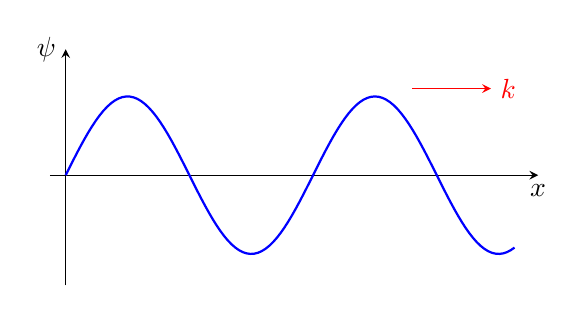
\begin{tikzpicture}[>=stealth]
      \draw[->] (-0.2,0)--(6.0,0) node[below]{$x$};
      \draw[->] (0,-1.4)--(0,1.6) node[left]{$\psi$};
      \draw[domain=0:5.7,samples=120,thick,blue] plot(\x,{sin(2*\x r)});
      \draw[->,red] (4.4,1.1)--(5.4,1.1) node[right]{$k$};
    \end{tikzpicture}
    \caption{Plane-wave profile and propagation vector.}
\end{figure}

\subsection*{Equations and Derivations}

The time-dependent Schrödinger wave equation for a free particle is

\begin{equation*}
i\hbar \frac{\partial \psi}{\partial t}
-\frac{\hbar^2}{2m}\nabla^2 \psi\qquad ...(1)
\end{equation*}

We assume a plane wave solution of the form

\begin{equation*}
\psi(\vec{r},t) = A e^{i(\vec{k}\cdot\vec{r} - \omega t)} \qquad ...(2)
\end{equation*}

where (A) is a constant amplitude.

Substituting Eq. (2) into Eq. (1), we obtain

\begin{equation*}
i\hbar (-i\omega)\psi
-\frac{\hbar^2}{2m}(-k^2)\psi\qquad ...(3)
\end{equation*}

Simplifying Eq. (3),

\begin{equation*}
\hbar \omega = \frac{\hbar^2 k^2}{2m}\qquad ...(4)
\end{equation*}

Using the relations

\begin{equation*}
E = \hbar \omega,\qquad\vec{p} = \hbar \vec{k}\qquad ...(5)
\end{equation*}

Eq. (4) becomes

\begin{equation*}
E = \frac{p^2}{2m}\qquad ...(6)
\end{equation*}

This is the classical expression for the kinetic energy of a free particle.

\subsection*{Final Expression}

\begin{equation*}
\boxed{\psi(\vec{r},t) = A e^{i(\vec{k}\cdot\vec{r} - \omega t)}}
\end{equation*}

This represents the plane wave solution of the Schrödinger wave equation.

\subsection*{Applications / Real-Life Examples}
The corresponding formulation is used in practical modeling and measurement workflows, including scattering analysis, spectroscopy, quantum-state calculations, and modern simulation pipelines in physics and engineering.

\subsection*{Conclusion}

A plane wave solution describes a free particle with definite energy and momentum. The wave function extends over all space and has constant probability density.

\section{Spin and Magnetic Moment of the Electron}



\subsection*{Theory}

In addition to orbital angular momentum, the electron possesses an intrinsic form of angular momentum known as spin. This intrinsic angular momentum is not associated with any classical motion of the electron in space. Corresponding to this spin angular momentum, the electron also possesses an intrinsic magnetic moment, which is responsible for its interaction with magnetic fields.


\subsection{Conceptual Explanation}
\textbf{Conceptual Explanation:} Electron spin is intrinsic angular momentum, not literal spatial rotation. Its associated magnetic moment explains Zeeman splitting, spin precession, and key spectroscopic signatures in electromagnetic fields.


\textbf{Advantage:} The spin--magnetic-moment framework explains fine structure, Zeeman splitting, and the outcome of spin-dependent measurements in atomic and condensed-matter systems.

\textbf{Limitation:} A purely classical picture of a spinning charged sphere is inadequate; the true origin of spin and its magnetic moment is intrinsically quantum mechanical.

\textbf{Conceptual Explanation:} Electron spin is intrinsic angular momentum, not literal spatial rotation. Its associated magnetic moment explains Zeeman splitting, spin precession, and key spectroscopic signatures in electromagnetic fields.

\subsection*{Important Diagram / Figure}

\begin{figure}[H]
    \centering
    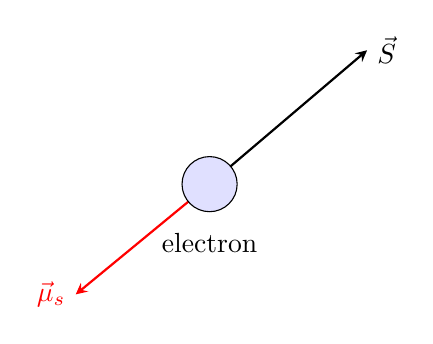
\begin{tikzpicture}[>=stealth]
      \draw[->,thick] (0,0)--(2.0,1.7) node[right] {$\vec{S}$};
      \draw[->,thick,red] (0,0)--(-1.7,-1.4) node[left] {$\vec{\mu}_s$};
      \draw[fill=blue!12] (0,0) circle (0.35);
      \node at (0,-0.75) {electron};
    \end{tikzpicture}
    \caption{Representation of electron spin and intrinsic magnetic moment vectors.}
\end{figure}

\subsection*{Important Diagram / Figure}
\begin{figure}[H]
    \centering
    \begin{tikzpicture}[>=stealth]
      \draw[->,thick] (0,0)--(0,3.0) node[above]{$\mathbf B$};
      \draw[->,thick,blue] (0,0)--(2.0,1.8) node[right]{$\mathbf S$};
      \draw[->,thick,red] (0,0)--(-1.6,-1.3) node[left]{$\boldsymbol\mu$};
    \end{tikzpicture}
    \caption{Spin and magnetic moment orientation in an external field.}
\end{figure}

\subsection*{Equations and Derivations}

The magnitude of the spin angular momentum of a particle is given by

\begin{equation*}
S = \sqrt{s(s+1)},\hbar \qquad ...(1)
\end{equation*}

where (s) is the spin quantum number.

For an electron, the spin quantum number is

\begin{equation*}
s = \frac{1}{2} \qquad ...(2)
\end{equation*}

Substituting Eq. (2) into Eq. (1), we obtain

\begin{equation*}
S = \sqrt{\frac{1}{2}\left(\frac{1}{2}+1\right)},\hbar= \sqrt{\frac{3}{4}},\hbar= \frac{\sqrt{3}}{2}\hbar\qquad ...(3)
\end{equation*}

The spin angular momentum vector ($\vec{S}$) is associated with a magnetic moment ($\vec{\mu}_s$), given by

\begin{equation*}
\vec{\mu}_s = -g \frac{e}{2m} \vec{S}\qquad ...(4)
\end{equation*}

where $e$ is the electronic charge, $m$ is the mass of the electron, and $g$ is the gyromagnetic ratio.

For the electron, the value of the gyromagnetic ratio is

\begin{equation*}
g \approx 2 \qquad ...(5)
\end{equation*}

Substituting Eq. (5) into Eq. (4), we get

\begin{equation*}
\vec{\mu}_s = - \frac{e}{m} \vec{S}\qquad ...(6)
\end{equation*}

The negative sign indicates that the direction of the magnetic moment is opposite to the direction of the spin angular momentum due to the negative charge of the electron.

\subsection*{Final Result / Expression}

\begin{equation*}
\boxed{\vec{\mu}_s = - \frac{e}{m} \vec{S}}
\end{equation*}

This expression represents the magnetic moment associated with the intrinsic spin of the electron.

\subsection*{Conclusion / Summary}

The electron possesses an intrinsic spin angular momentum equal to ($\frac{1}{2}\hbar$), independent of its orbital motion. The associated magnetic moment explains the magnetic behaviour of electrons and plays a fundamental role in atomic and quantum phenomena.

\section{Properties of gamma-matrices}



\subsection*{Theory}

The $\gamma$-matrices are a set of matrices introduced in the Dirac equation to ensure its relativistic covariance and linearity in both space and time derivatives. These matrices satisfy specific algebraic relations which are necessary for consistency with the relativistic energy--momentum relation.


\subsection{Conceptual Explanation}
\textbf{Conceptual Explanation:} Gamma matrices realize relativistic spinor algebra and enforce Lorentz-compatible dynamics in the Dirac theory. Their anticommutation structure guarantees the correct relativistic energy-momentum relation.


They form a set of four matrices $\gamma^\mu$ ($$\mu = 0,1,2,3$$) that obey definite anticommutation relations, known as the Dirac algebra.

\subsection*{Important Diagram / Figure}

\begin{figure}[H]
    \centering
    \includegraphics[width=0.55\textwidth]{uploads/ch2_docx_image1.png}
    \caption{Schematic Representation of Dirac $\gamma$-Matrices}
\end{figure}

Figure: Schematic representation of ($4 \times 4$) Dirac $\gamma$-matrices and their algebraic structure.

\subsection*{Equations and Derivations}

\subsection*{Anticommutation Relations}

The fundamental property of the $\gamma$-matrices is given by

\begin{equation*}
{ \gamma^\mu , \gamma^\nu }
\gamma^\mu \gamma^\nu + \gamma^\nu \gamma^\mu
\gamma^\mu \gamma^\nu + \gamma^\nu \gamma^\mu = 2g^{\mu\nu} I\qquad ...(1)
\end{equation*}

where

$g^{\mu\nu}$ is the metric tensor, and $I$ is the unit matrix.

This relation defines the Dirac algebra.

\subsection*{Square of $\gamma$-Matrices}

From Eq. (1), for ($ \mu = \nu $),

\begin{equation*}
(\gamma^\mu)^2 = g^{\mu\mu} I\qquad ...(2)
\end{equation*}

Thus,

\begin{equation*}
(\gamma^0)^2 = I,\qquad(\gamma^i)^2 = -I \quad (i = 1,2,3)\qquad ...(3)
\end{equation*}

\subsection*{Hermitian Properties}

The Hermitian conjugates of the $\gamma$-matrices satisfy

\begin{equation*}
(\gamma^0)^\dagger = \gamma^0\qquad ...(4)
\end{equation*}

\begin{equation*}
(\gamma^i)^\dagger = -\gamma^i\qquad ...(5)
\end{equation*}

These relations ensure that the Dirac Hamiltonian is Hermitian.

\subsection*{Trace Properties}

The trace of a single $\gamma$-matrix is zero:

\begin{equation*}
\text{Tr}(\gamma^\mu) = 0\qquad ...(6)
\end{equation*}

Also,

\begin{equation*}
\text{Tr}(\gamma^\mu \gamma^\nu) = 4 g^{\mu\nu}\qquad ...(7)
\end{equation*}

These relations are useful in evaluating physical quantities.

\subsection*{Commutation Relations}

The commutator of $\gamma$-matrices is defined as

\begin{equation*}
[\gamma^\mu , \gamma^\nu] = \gamma^\mu \gamma^\nu - \gamma^\nu \gamma^\mu\qquad ...(8)
\end{equation*}

From this, one defines the matrices

\begin{equation*}
\sigma^{\mu\nu}
\frac{i}{2}[\gamma^\mu , \gamma^\nu]\qquad ...(9)
\end{equation*}

which are associated with spin and Lorentz transformations.

\subsection*{Product Relations}

The product of different $\gamma$-matrices satisfies

\begin{equation*}
\gamma^\mu \gamma^\nu = - \gamma^\nu \gamma^\mu\quad \text{for } \mu \neq \nu\qquad ...(10)
\end{equation*}

This follows directly from the anticommutation relation.

\subsection*{Definition of $\gamma^5$}

An important matrix is defined as

\begin{equation*}
\gamma^5 = i \gamma^0 \gamma^1 \gamma^2 \gamma^3\qquad ...(11)
\end{equation*}

It satisfies

\begin{equation*}
(\gamma^5)^2 = I\qquad ...(12)
\end{equation*}

and

\begin{equation*}
{ \gamma^5 , \gamma^\mu } = 0\qquad ...(13)
\end{equation*}

\subsection*{Lorentz Covariance Condition}

The $\gamma$-matrices satisfy transformation properties such that the Dirac equation remains invariant under Lorentz transformations. This requirement leads to constraints consistent with Eq. (1), ensuring relativistic covariance .

\subsection*{Final Expression}

\begin{equation*}
\boxed{
{ \gamma^\mu , \gamma^\nu }
\gamma^\mu \gamma^\nu + \gamma^\nu \gamma^\mu = 2g^{\mu\nu} I}
\end{equation*}

This relation defines the complete algebraic structure of the $\gamma$-matrices.

\subsection*{Applications / Real-Life Examples}
The corresponding formulation is used in practical modeling and measurement workflows, including scattering analysis, spectroscopy, quantum-state calculations, and modern simulation pipelines in physics and engineering.

\subsection*{Conclusion}

The $\gamma$-matrices satisfy specific anticommutation, Hermitian, and trace relations that ensure the consistency of the Dirac equation with relativity. These properties form the mathematical foundation of relativistic quantum mechanics for spin-($\tfrac{1}{2}$) particles.

\section{Spin and Magnetic Moment of the Electron}



\subsection*{Theory}

In addition to orbital angular momentum, the electron possesses an intrinsic form of angular momentum known as spin. This intrinsic angular momentum is not associated with any classical motion of the electron in space. Corresponding to this spin angular momentum, the electron also possesses an intrinsic magnetic moment, which is responsible for its interaction with magnetic fields.


\subsection{Conceptual Explanation}
\textbf{Conceptual Explanation:} Electron spin is intrinsic angular momentum, not literal spatial rotation. Its associated magnetic moment explains Zeeman splitting, spin precession, and key spectroscopic signatures in electromagnetic fields.


\textbf{Advantage:} The spin--magnetic-moment framework explains fine structure, Zeeman splitting, and the outcome of spin-dependent measurements in atomic and condensed-matter systems.

\textbf{Limitation:} A purely classical picture of a spinning charged sphere is inadequate; the true origin of spin and its magnetic moment is intrinsically quantum mechanical.

\textbf{Conceptual Explanation:} Electron spin is intrinsic angular momentum, not literal spatial rotation. Its associated magnetic moment explains Zeeman splitting, spin precession, and key spectroscopic signatures in electromagnetic fields.

\subsection*{Important Diagram / Figure}

\begin{figure}[H]
    \centering
    \includegraphics[width=0.72\textwidth]{spin-magnetic-moment-electron.png}
    \caption{Representation of electron spin and magnetic moment vectors.}
\end{figure}

\subsection*{Equations and Derivations}

The magnitude of the spin angular momentum of a particle is given by

\begin{equation*}
S = \sqrt{s(s+1)},\hbar \qquad ...(1)
\end{equation*}

where (s) is the spin quantum number.

For an electron, the spin quantum number is

\begin{equation*}
s = \frac{1}{2} \qquad ...(2)
\end{equation*}

Substituting Eq. (2) into Eq. (1), we obtain

\begin{equation*}
S = \sqrt{\frac{1}{2}\left(\frac{1}{2}+1\right)},\hbar= \sqrt{\frac{3}{4}},\hbar= \frac{\sqrt{3}}{2}\hbar\qquad ...(3)
\end{equation*}

The spin angular momentum vector ($\vec{S}$) is associated with a magnetic moment ($\vec{\mu}_s$), given by

\begin{equation*}
\vec{\mu}_s = -g \frac{e}{2m} \vec{S}\qquad ...(4)
\end{equation*}

where $e$ is the electronic charge, $m$ is the mass of the electron, and $g$ is the gyromagnetic ratio.

For the electron, the value of the gyromagnetic ratio is

\begin{equation*}
g \approx 2 \qquad ...(5)
\end{equation*}

Substituting Eq. (5) into Eq. (4), we get

\begin{equation*}
\vec{\mu}_s = - \frac{e}{m} \vec{S}\qquad ...(6)
\end{equation*}

The negative sign indicates that the direction of the magnetic moment is opposite to the direction of the spin angular momentum due to the negative charge of the electron.

\subsection*{Final Expression}

\begin{equation*}
\boxed{\vec{\mu}_s = - \frac{e}{m} \vec{S}}
\end{equation*}

This expression represents the magnetic moment associated with the intrinsic spin of the electron.

\subsection*{Applications / Real-Life Examples}
The corresponding formulation is used in practical modeling and measurement workflows, including scattering analysis, spectroscopy, quantum-state calculations, and modern simulation pipelines in physics and engineering.

\subsection*{Conclusion}

The electron possesses an intrinsic spin angular momentum equal to ($\frac{1}{2}\hbar$), independent of its orbital motion. The associated magnetic moment explains the magnetic behaviour of electrons and plays a fundamental role in atomic and quantum phenomena.

\section{Normalisation and Completeness of Spinors}



\subsection*{Theory}

In relativistic quantum mechanics, the solutions of the Dirac equation are expressed in the form of multi-component wave functions known as spinors. For these spinors to represent physically acceptable states, they must satisfy suitable normalisation conditions so that probabilities remain finite and well-defined. In addition, the complete set of spinor solutions must obey a completeness relation, which ensures that any arbitrary state of the system can be expanded as a linear combination of these basic spinor states.


\subsection{Conceptual Explanation}
\textbf{Conceptual Explanation:} Normalization fixes probabilistic interpretation of spinor states, while completeness ensures expansion of physical fermionic states in a full basis. Together they make scattering and field quantization calculations consistent.


\subsection*{Important Diagram / Figure}

\begin{figure}[H]
    \centering
    \includegraphics[width=0.78\textwidth]{spinor-poincare-sphere.png}
    \caption{Schematic representation of spinor evolution using the Poincar\'e sphere.}
\end{figure}


\subsection*{Equations and Derivations}

Let $u_r(\vec{p})$ denote the positive-energy spinors and $v_r(\vec{p})$ denote the negative-energy spinors corresponding to a particle with momentum $\vec{p}$. The index $r$ labels the spin states.

\subsection*{Normalisation of Positive-Energy Spinors}

The normalisation condition for the positive-energy spinors is defined as

\begin{equation*}
u_r^\dagger(\vec{p}), u_s(\vec{p}) = \delta_{rs}\qquad ...(1)
\end{equation*}

where($\delta_{rs}$) is the Kronecker delta, equal to unity when (r = s) and zero otherwise.

Equation (1) ensures that spinors corresponding to different spin states are orthonormal.

\subsection*{Normalisation of Negative-Energy Spinors}

Similarly, the negative-energy spinors satisfy the condition

\begin{equation*}
v_r^\dagger(\vec{p}), v_s(\vec{p}) = \delta_{rs}\qquad ...(2)
\end{equation*}

This relation guarantees that negative-energy states are also properly normalised and mutually orthogonal.

\subsection*{Orthogonality of Positive- and Negative-Energy Spinors}

The orthogonality between positive- and negative-energy solutions is expressed as

\begin{equation*}
u_r^\dagger(\vec{p}), v_s(\vec{p}) = 0\qquad ...(3)
\end{equation*}

Equation (3) shows that particle and antiparticle spinor states are independent of each other.

\subsection*{Completeness Relation}

The completeness of the full set of spinor solutions is expressed by the relation

\begin{equation*}
\sum_r \left[ u_r(\vec{p}), u_r^\dagger(\vec{p})
v_r(\vec{p}), v_r^\dagger(\vec{p}) \right] = I\qquad ...(4)
\end{equation*}

where $I$ is the unit matrix in spinor space.

This relation states that the combined set of positive- and negative-energy spinors forms a complete basis. Any arbitrary four-component spinor ($\psi$) can therefore be expanded in terms of $u_r$ and $v_r$.

\subsection*{Physical Significance of Completeness}

The completeness relation ensures that no physically relevant state lies outside the space spanned by the Dirac spinors. It is essential for constructing general solutions of the Dirac equation and for evaluating physical quantities expressed as matrix elements.

\subsection*{Final Expression}

\begin{equation*}
\boxed{\sum_r \left[ u_r(\vec{p}), u_r^\dagger(\vec{p})
v_r(\vec{p}), v_r^\dagger(\vec{p}) \right] = I}
\end{equation*}

This equation represents the completeness condition for relativistic spinors.

\subsection*{Applications / Real-Life Examples}
The corresponding formulation is used in practical modeling and measurement workflows, including scattering analysis, spectroscopy, quantum-state calculations, and modern simulation pipelines in physics and engineering.

\subsection*{Conclusion}

The normalisation conditions ensure that individual spinor states possess a consistent probabilistic interpretation, while the completeness relation guarantees that the full set of spinors spans the entire state space. Together, these properties form a fundamental mathematical foundation for the relativistic description of spin-($\tfrac{1}{2}$) particles.

\section{Existence of Electron Spin}



\subsection*{Theory}

The existence of electron spin refers to the presence of an intrinsic angular momentum associated with the electron, independent of its orbital motion. This intrinsic angular momentum is a fundamental property of the electron and arises naturally within the framework of relativistic quantum mechanics. The concept of electron spin is necessary to account for several physical phenomena that cannot be explained by orbital angular momentum alone.


\subsection{Conceptual Explanation}
\textbf{Conceptual Explanation:} Electron spin follows from relativistic quantum theory and experimental evidence such as fine structure and Stern–Gerlach-type effects. It is a fundamental internal degree of freedom required by nature.



\subsection*{Important Diagram / Figure}
\begin{figure}[H]
    \centering
    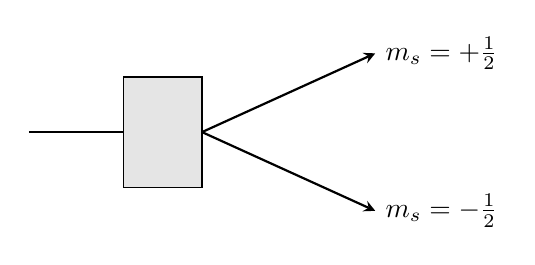
\begin{tikzpicture}[>=stealth]
      \draw[thick](0,0)--(2.2,0);
      \draw[fill=gray!20](1.2,-0.7) rectangle (2.2,0.7);
      \draw[->,thick](2.2,0)--(4.4,1.0) node[right]{$m_s=+\frac12$};
      \draw[->,thick](2.2,0)--(4.4,-1.0) node[right]{$m_s=-\frac12$};
    \end{tikzpicture}
    \caption{Stern--Gerlach splitting and quantized spin projection.}
\end{figure}

\subsection*{Equations and Derivations}

In classical mechanics, the angular momentum of a particle is given by

\begin{equation*}
\vec{L} = \vec{r} \times \vec{p}\qquad ...(1)
\end{equation*}

However, this expression alone is insufficient to describe the total angular momentum of an electron.

In relativistic quantum mechanics, the total angular momentum operator is defined as

\begin{equation*}
\vec{J} = \vec{L} + \vec{S}\qquad ...(2)
\end{equation*}

where($\vec{L}$) is the orbital angular momentum operator, and($\vec{S}$) is the intrinsic spin angular momentum operator.

The components of the spin angular momentum satisfy the commutation relations

\begin{equation*}
[S_i, S_j] = i\hbar \epsilon_{ijk} S_k\qquad ...(3)
\end{equation*}

which are identical in form to those satisfied by orbital angular momentum operators.

The magnitude of the spin angular momentum is given by

\begin{equation*}
S = \sqrt{s(s+1)},\hbar\qquad ...(4)
\end{equation*}

For the electron, the spin quantum number is

\begin{equation*}
s = \frac{1}{2}\qquad ...(5)
\end{equation*}

Substituting Eq. (5) into Eq. (4), we obtain

\begin{equation*}
S = \sqrt{\frac{1}{2}\left(\frac{1}{2}+1\right)},\hbar= \frac{\sqrt{3}}{2}\hbar\qquad ...(6)
\end{equation*}

This result shows that the electron possesses a definite intrinsic angular momentum even in the absence of orbital motion.

\subsection*{Relativistic Origin of Spin}

The Dirac equation for a free electron is a first-order relativistic wave equation. Its solutions are four-component spinors, which inherently describe two independent spin states for positive energy solutions and two for negative energy solutions.

The appearance of these multiple components directly leads to the interpretation that the electron possesses intrinsic spin. This feature emerges naturally from the algebra of the Dirac matrices and does not require any additional postulate .

\subsection*{Experimental Evidence}

Experimental observations such as the splitting of spectral lines in a magnetic field and the behavior of electrons in Stern--Gerlach type experiments provide direct confirmation of the existence of electron spin. These effects require the presence of an intrinsic magnetic moment associated with spin, which cannot be attributed to orbital motion alone .

\subsection*{Final Expression}

\begin{equation*}
\boxed{\vec{J} = \vec{L} + \vec{S}, \qquad s = \frac{1}{2}}
\end{equation*}

This result establishes that the total angular momentum of the electron consists of both orbital and intrinsic spin contributions.

\subsection*{Applications / Real-Life Examples}
The corresponding formulation is used in practical modeling and measurement workflows, including scattering analysis, spectroscopy, quantum-state calculations, and modern simulation pipelines in physics and engineering.

\subsection*{Conclusion}

The existence of electron spin is a fundamental consequence of relativistic quantum mechanics and is confirmed by experimental evidence. It represents an intrinsic angular momentum of the electron, independent of orbital motion, and is essential for a complete description of atomic and subatomic phenomena.


\chapter{Quantum Field Theory}

\section{Lagrangian field theory}



\begin{figure}[H]
    \centering
    \includegraphics[width=0.72\textwidth]{prism-uploads/field_theory_1.png}
    \caption{Lagrangian Field Theory Diagram}
\end{figure}

\subsection*{Theory}
A physical system with infinitely many (uncountable) degrees of freedom is called a field. In field theory, the dynamical variable is a function such as $\psi(\mathbf{r},t)$ defined at every point in space and time. Thus, field theory extends finite-dimensional classical mechanics into a continuous setting. The field carries energy, momentum, angular momentum, and other observables.


\subsection{Conceptual Explanation}
\textbf{Conceptual Explanation:} Lagrangian field theory encodes dynamics via an action principle. Symmetries of the Lagrangian generate conservation laws, giving a unified and systematic route to equations of motion.


In the variational formulation, one introduces a Lagrangian density $\mathcal{L}$ and obtains equations of motion by demanding stationarity of the action. This parallels the particle case, but with space and time integrations replacing sums over discrete coordinates.

\subsection*{Important Diagram / Figure}
The associated derivation is primarily analytic and variational; the supporting diagram is included for conceptual reference.

\subsection*{Equations and Derivations}
Starting from Hamilton's variational principle,
\begin{equation}
\delta \int_{t_1}^{t_2} L\,dt = 0,
\qquad
\delta\psi(\mathbf{r},t_1)=\delta\psi(\mathbf{r},t_2)=0.
\end{equation}
Define the field Lagrangian:
\begin{equation}
L = \int \mathcal{L}(\psi,\nabla\psi,\dot\psi,t)\,d\tau.
\end{equation}
Variation of $\mathcal{L}$ gives
\begin{equation}
\delta\mathcal{L}=\frac{\partial\mathcal{L}}{\partial\psi}\delta\psi
+\sum_{k=1}^{3}\frac{\partial\mathcal{L}}{\partial(\partial\psi/\partial x_k)}\delta\left(\frac{\partial\psi}{\partial x_k}\right)
+\frac{\partial\mathcal{L}}{\partial\dot\psi}\delta\dot\psi.
\end{equation}
Using
\begin{equation}
\delta\left(\frac{\partial\psi}{\partial x_k}\right)=\frac{\partial}{\partial x_k}(\delta\psi),
\qquad
\delta\dot\psi=\frac{\partial}{\partial t}(\delta\psi),
\end{equation}
and integrating by parts in space and time (surface terms vanish with standard boundary conditions), we obtain
\begin{equation}
\frac{\partial\mathcal{L}}{\partial\psi}
-\sum_{k=1}^{3}\frac{\partial}{\partial x_k}\left(\frac{\partial\mathcal{L}}{\partial(\partial\psi/\partial x_k)}\right)
-\frac{\partial}{\partial t}\left(\frac{\partial\mathcal{L}}{\partial\dot\psi}\right)=0.
\end{equation}

\subsection*{Final Expression}
\begin{equation}
\boxed{\frac{\partial\mathcal{L}}{\partial\psi}
-\sum_{k=1}^{3}\frac{\partial}{\partial x_k}\left(\frac{\partial\mathcal{L}}{\partial(\partial\psi/\partial x_k)}\right)
-\frac{\partial}{\partial t}\left(\frac{\partial\mathcal{L}}{\partial\dot\psi}\right)=0}
\end{equation}

\subsection*{Applications / Real-Life Examples}
The corresponding formulation is used in practical modeling and measurement workflows, including scattering analysis, spectroscopy, quantum-state calculations, and modern simulation pipelines in physics and engineering.

\subsection*{Conclusion}
This is the Euler--Lagrange field equation, the continuous-field analogue of classical Lagrange equations.

\section{Hamiltonian formulation}



\subsection*{Theory}
For field quantization, it is useful to pass to Hamiltonian form. The pair $\psi(\mathbf{r},t)$ and conjugate momentum density $\pi(\mathbf{r},t)$ play roles analogous to generalized coordinates and momenta.


\subsection{Conceptual Explanation}
\textbf{Conceptual Explanation:} Hamiltonian formulation reorganizes dynamics in terms of fields and conjugate momenta, highlighting energy structure and canonical evolution. It is the natural starting point for canonical quantization.


\subsection*{Important Diagram / Figure}
\begin{figure}[H]
    \centering
    \includegraphics[width=0.72\textwidth]{prism-uploads/field_theory_2.png}
    \caption{Hamiltonian Formulation Diagram}
\end{figure}

\subsection*{Equations and Derivations}
\begin{equation}
\pi(\mathbf{r},t)=\frac{\partial\mathcal{L}}{\partial\dot\psi(\mathbf{r},t)}.
\end{equation}
\begin{equation}
\mathcal{H}(\psi,\pi)=\pi\dot\psi-\mathcal{L},
\qquad
H=\int\mathcal{H}\,d\tau.
\end{equation}
By comparing arbitrary variations $\delta L$ and $\delta H$, one gets
\begin{equation}
\dot\psi=\frac{\bar\partial H}{\bar\partial\pi},
\qquad
\dot\pi=-\frac{\bar\partial H}{\bar\partial\psi}.
\end{equation}

\subsection*{Conclusion}
The Hamiltonian functional generates complete field evolution in phase-space form.

\section{Quantization of scalar fields}



\subsection*{Theory}
Canonical quantization promotes classical fields and conjugate momenta to operators and imposes equal-time commutators.


\subsection{Conceptual Explanation}
\textbf{Conceptual Explanation:} Quantizing scalar fields promotes classical modes to operators that create and annihilate particles. This turns wave excitations into particle quanta with relativistic dispersion and vacuum structure.


\subsection*{Important Diagram / Figure}
\begin{figure}[H]
    \centering
    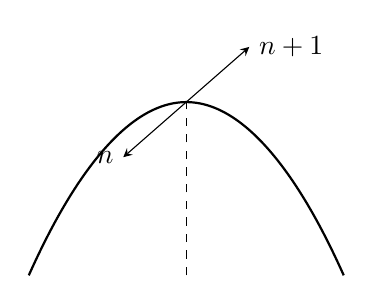
\begin{tikzpicture}[>=stealth]
      \draw[thick] (0,0) parabola bend (2,2.2) (4,0);
      \draw[dashed] (2,0) -- (2,2.2);
      \draw[->] (2,2.2) -- (2.8,2.9) node[right] {$n+1$};
      \draw[->] (2,2.2) -- (1.2,1.5) node[left] {$n$};
    \end{tikzpicture}
    \caption{Ladder-operator picture used in scalar-field quantization.}
\end{figure}

\begin{figure}[H]
    \centering
    \includegraphics[width=0.78\textwidth]{quantization-scalar-field-diagram.png}
    \caption{Additional diagram for quantization of the scalar field.}
\end{figure}

\subsection*{Equations and Derivations}
Discretizing space into cells and taking the continuum limit:
\begin{equation}
[\psi_i,\pi_j]=i\hbar\frac{\delta_{ij}}{\Delta\tau_j}
\quad\Longrightarrow\quad
[\psi(\mathbf{r},t),\pi(\mathbf{r}',t)]=i\hbar\delta(\mathbf{r}-\mathbf{r}').
\end{equation}
Also,
\begin{equation}
[\psi(\mathbf{r},t),\psi(\mathbf{r}',t)]=0,
\qquad
[\pi(\mathbf{r},t),\pi(\mathbf{r}',t)]=0.
\end{equation}
These relations define the canonical operator algebra for bosonic scalar fields.

\subsection*{Conclusion}
The commutator structure is the foundation for second-quantized scalar dynamics.

\section{Quantization of complex scalar and Schr"odinger fields}



\subsection*{Theory}
Complex scalar fields naturally encode particles and antiparticles. Schr"odinger fields provide the non-relativistic second-quantized framework with field operators acting on Fock states.


\subsection{Conceptual Explanation}
\textbf{Conceptual Explanation:} Complex-field quantization separates particle and antiparticle degrees of freedom and introduces conserved charge. It connects nonrelativistic Schrödinger fields to many-body operator language.


\subsection*{Important Diagram / Figure}
\begin{figure}[H]
    \centering
    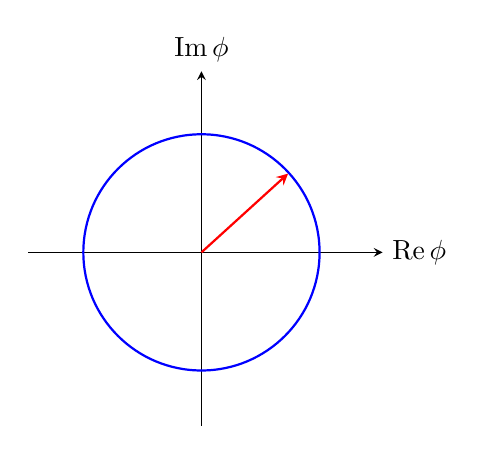
\begin{tikzpicture}[>=stealth]
      \draw[->] (-2.2,0)--(2.3,0) node[right]{Re$\,\phi$};
      \draw[->] (0,-2.2)--(0,2.3) node[above]{Im$\,\phi$};
      \draw[thick,blue](0,0) circle (1.5);
      \draw[->,red,thick](0,0)--(1.1,1.0);
    \end{tikzpicture}
    \caption{Complex scalar field phase rotation in the complex plane.}
\end{figure}

\begin{figure}[!htbp]
    \centering
    \includegraphics[width=0.78\textwidth]{complex-scalar-real-imag-r025.png}
    \caption{Real versus imaginary parts of the complex scalar field at $r=0.25$.}
\end{figure}

\subsection*{Equations and Derivations}
A complex scalar field may be expanded as
\begin{equation}
\phi(x)=\sum_k\left(a_k e^{-ikx}+b_k^{\dagger}e^{ikx}\right),
\end{equation}
where $a_k$ annihilates particle modes and $b_k^{\dagger}$ creates antiparticle modes.
For Schr"odinger fields,
\begin{equation}
i\hbar\frac{\partial\psi}{\partial t}=\left(-\frac{\hbar^2}{2m}\nabla^2+V\right)\psi,
\qquad
\pi=i\hbar\psi^{\dagger}.
\end{equation}
This operator formalism reproduces many-particle quantum mechanics while allowing variable particle number.

\subsection*{Final Expression}
\begin{equation}
\boxed{\phi(x)=\sum_k\left(a_k e^{-ikx}+b_k^{\dagger}e^{ikx}\right)}
\end{equation}

\subsection*{Applications / Real-Life Examples}
The corresponding formulation is used in practical modeling and measurement workflows, including scattering analysis, spectroscopy, quantum-state calculations, and modern simulation pipelines in physics and engineering.

\subsection*{Conclusion}
Quantized complex and Schr"odinger fields describe creation/annihilation processes in relativistic and non-relativistic limits.

\section{Bosons and fermions}



\subsection*{Theory}
Particles are classified through intrinsic spin and exchange symmetry. This classification determines the statistics and allowed occupation properties of many-body states.


\subsection{Conceptual Explanation}
\textbf{Conceptual Explanation:} Bosons and fermions differ by exchange symmetry, leading to Bose enhancement and Pauli exclusion respectively. These statistics govern collective behavior from lasers and condensates to atomic structure.


\subsection*{Important Diagram / Figure}
\begin{figure}[H]
    \centering
    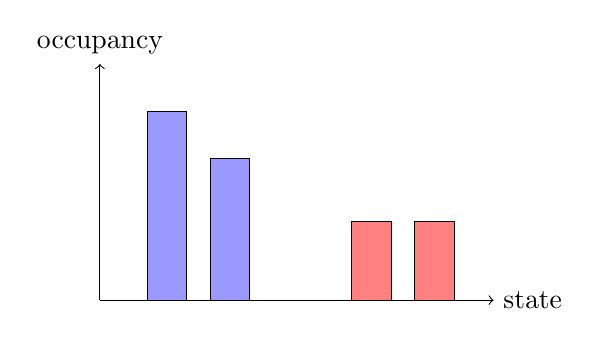
\begin{tikzpicture}
      \draw[->](0,0)--(5.0,0) node[right]{state};
      \draw[->](0,0)--(0,3.0) node[above]{occupancy};
      \draw[fill=blue!40](0.6,0) rectangle (1.1,2.4);
      \draw[fill=blue!40](1.4,0) rectangle (1.9,1.8);
      \draw[fill=red!50](3.2,0) rectangle (3.7,1.0);
      \draw[fill=red!50](4.0,0) rectangle (4.5,1.0);
    \end{tikzpicture}
    \caption{Bosonic multi-occupancy versus fermionic exclusion (schematic).}
\end{figure}

\begin{figure}[!htbp]
    \centering
    \includegraphics[width=0.80\textwidth]{degenerate-bosons-fermions-sun.png}
    \caption{Degenerate bosons, fermions, and SUN fermions.}
\end{figure}

\subsection*{Equations and Derivations}
\begin{equation}
|\mathbf{S}|=\sqrt{s(s+1)}\hbar.
\end{equation}
Fermions have half-integer spin:
\begin{equation}
s=\frac12,\frac32,\dots,
\end{equation}
and follow Fermi--Dirac statistics (antisymmetric states).
Bosons have integer spin:
\begin{equation}
s=0,1,2,\dots,
\end{equation}
and follow Bose--Einstein statistics (symmetric states).

\subsection*{Conclusion}
The spin-statistics connection separates elementary quanta into fermionic and bosonic sectors.

\section{Klein--Gordon field}



\subsection*{Theory}
The Klein--Gordon equation is the relativistic wave equation for scalar (spin-0) particles, obtained by combining quantum-operator substitutions with the relativistic energy--momentum relation.


\subsection{Conceptual Explanation}
\textbf{Conceptual Explanation:} The Klein–Gordon field is the relativistic theory of spin-0 particles. It provides the prototype for covariant quantization, propagators, and causality analysis in quantum field theory.


\subsection*{Important Diagram / Figure}

\begin{figure}[!htbp]
    \centering
    \includegraphics[width=0.72\textwidth]{klein-gordon 1.png}
    \caption{Klein--Gordon field diagram I.}
\end{figure}

\begin{figure}[!htbp]
    \centering
    \includegraphics[width=0.72\textwidth]{klein-gordon 2.png}
    \caption{Klein--Gordon field diagram II.}
\end{figure}

\subsection*{Equations and Derivations}
\begin{equation}
E^2=p^2c^2+m^2c^4,
\qquad
E\to i\hbar\frac{\partial}{\partial t},
\quad
\mathbf{p}\to -i\hbar\nabla.
\end{equation}
Hence,
\begin{equation}
\left(\frac{1}{c^2}\frac{\partial^2}{\partial t^2}-\nabla^2+\frac{m^2c^2}{\hbar^2}\right)\psi=0.
\end{equation}
With the d'Alembertian,
\begin{equation}
\Box\equiv\frac{1}{c^2}\frac{\partial^2}{\partial t^2}-\nabla^2,
\qquad
(\Box+\frac{m^2c^2}{\hbar^2})\psi=0.
\end{equation}
A plane-wave solution $\psi=Ae^{i(\mathbf{p}\cdot\mathbf{x}-Et)/\hbar}$ satisfies the same dispersion relation. Field densities are
\begin{equation}
\mathcal{L}=\frac12\left(\partial_\mu\phi\,\partial^\mu\phi-m^2\phi^2\right),
\qquad
\mathcal{H}=\frac12\left(\pi^2+(\nabla\phi)^2+m^2\phi^2\right).
\end{equation}

\subsection*{Final Expression}
\begin{equation}
\boxed{\left(\Box+\frac{m^2c^2}{\hbar^2}\right)\psi=0}
\end{equation}

\subsection*{Applications / Real-Life Examples}
The corresponding formulation is used in practical modeling and measurement workflows, including scattering analysis, spectroscopy, quantum-state calculations, and modern simulation pipelines in physics and engineering.

\subsection*{Conclusion}
The Klein--Gordon field is Lorentz invariant and forms a core building block for relativistic scalar quantum theory.

\section{Dirac field}



\subsection*{Theory}
The Dirac field describes relativistic spin-$\frac12$ particles with spinor wave functions and guarantees Lorentz covariance through the $\gamma^\mu$-matrix algebra.


\subsection{Conceptual Explanation}
\textbf{Conceptual Explanation:} The Dirac field describes spin-1/2 matter with built-in relativistic covariance and antiparticles. Its structure explains spin, magnetic moments, and conserved currents in fermionic interactions.


\subsection*{Important Diagram / Figure}
\begin{figure}[H]
    \centering
    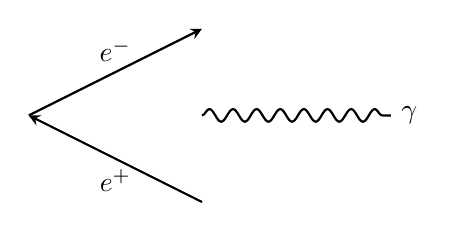
\begin{tikzpicture}[>=stealth]
      \draw[thick,->](0,0)--(2.2,1.1) node[midway,above]{$e^-$};
      \draw[thick,->](2.2,-1.1)--(0,0) node[midway,below]{$e^+$};
      \draw[decorate,decoration={snake,amplitude=0.8mm,segment length=3mm},thick](2.2,0)--(4.6,0) node[right]{$\gamma$};
    \end{tikzpicture}
    \caption{Fermion-antifermion interaction schematic for Dirac-field processes.}
\end{figure}

\begin{figure}[!htbp]
    \centering
    \includegraphics[width=0.72\textwidth]{dirac-field.png}
    \caption{Dirac field illustration I.}
\end{figure}

\begin{figure}[!htbp]
    \centering
    \includegraphics[width=0.72\textwidth]{dirac-field-2.png}
    \caption{Dirac field illustration II.}
\end{figure}

\subsection*{Equations and Derivations}
\begin{equation}
\left(i\gamma^\mu\partial_\mu-\frac{mc}{\hbar}\right)\psi=0,
\qquad
\partial_\mu\bar\psi\,i\gamma^\mu+\frac{mc}{\hbar}\bar\psi=0.
\end{equation}
\begin{equation}
\mathcal{L}=\hbar c\,\bar\psi\left(i\gamma^\mu\partial_\mu-\frac{mc}{\hbar}\right)\psi.
\end{equation}
\begin{equation}
E^{\mu\nu}=\hbar c\,\bar\psi\gamma^\nu\partial^\mu\psi+g^{\mu\nu}\mathcal{L},
\qquad
\Theta^{\mu\nu}=\frac12\left(E^{\mu\nu}+E^{\nu\mu}\right).
\end{equation}
Momentum-space projection operators are
\begin{equation}
\Lambda_{\pm}=\frac{1}{2mc}\left(mc\pm i\gamma^\mu p_\mu\right),
\qquad
\xi=\xi_++\xi_-,\;\xi_\pm=\Lambda_\pm\xi.
\end{equation}

\subsection*{Final Expression}
\begin{equation}
\boxed{\Lambda_{\pm}=\frac{1}{2mc}\left(mc\pm i\gamma^\mu p_\mu\right)}
\end{equation}

\subsection*{Applications / Real-Life Examples}
The corresponding formulation is used in practical modeling and measurement workflows, including scattering analysis, spectroscopy, quantum-state calculations, and modern simulation pipelines in physics and engineering.

\subsection*{Conclusion}
Dirac field equations, energy-momentum tensors, and spinor projectors together provide the relativistic quantum framework for fermionic matter.


\chapter{Quantum Chromodynamics I}

\section{Introduction to Quantum Chromodynamics (QCD)}



\subsection*{Theory}
Modern particle physics seeks to understand the fundamental constituents of matter and the forces governing their interactions. Among these, the strong interaction, described by Quantum Chromodynamics (QCD), plays a crucial role in binding quarks into hadrons such as protons and neutrons. QCD is the theory that describes the action of the strong force.


\subsection{Conceptual Explanation}
\textbf{Conceptual Explanation:} QCD is the non-Abelian gauge theory of strong interactions, with quarks interacting through gluons and color charge. Confinement and asymptotic freedom explain hadronic structure across energy scales.


QCD was constructed in analogy to Quantum Electrodynamics (QED), the quantum field theory of the electromagnetic force. In QED, interactions of charged particles occur through the emission and absorption of massless photons (force carriers). By analogy, QCD predicts force-carrier particles called gluons, which transmit the strong force between particles carrying color charge. Therefore, the strong force acts on quarks and composite particles built from quarks, such as protons, neutrons, and mesons.

The concept of color as the source of a strong field was developed into the QCD framework in 1973 by Harald Fritzsch, Heinrich Leutwyler, and Murray Gell-Mann. Unlike photons in QED, gluons carry color charge and can interact with each other, a non-Abelian feature rooted in Yang--Mills gauge theory.

\subsection{Color Charge}
While QED has one type of electric charge (with charge/anticharge), QCD requires three types of color charge to explain quark behavior: red, green, and blue (names only, with no visual meaning). Each has a corresponding anticolor.

\subsection{Key Features of QCD}
\begin{itemize}
    \item QCD describes strong interactions through quark--gluon dynamics.
    \item It is a non-Abelian gauge theory with symmetry group $SU(3)$.
    \item It has 8 gluons as force carriers.
    \item Because gluons carry color, they interact with each other.
    \item Its compact gauge-theory form leads to rich phenomena: running coupling, hadronization, and confinement.
\end{itemize}

\subsection{Perturbative QCD}
Perturbative methods are suitable at very high energies, where the coupling is weak. They are used to calculate cross-sections for processes such as top-quark production and searches for new particles at colliders.

At short distances, asymptotic freedom makes fixed-order expansions reliable. In practice, one combines partonic amplitudes with parton distribution functions to predict hadronic observables.

\begin{figure}[H]
    \centering
    \includegraphics[width=0.72\textwidth]{fig_4_1_4_perturbative_qcd.png}
    \caption{Illustrative diagram for perturbative QCD processes.}
    \label{fig:perturbative-qcd-diagram}
\end{figure}

\subsection{Asymptotic Freedom and Confinement}
\begin{itemize}
    \item \textbf{Asymptotic freedom:} At short distances (high energies), quarks and gluons behave approximately as free particles.
    \item \textbf{Confinement:} At low energies, quarks are tightly bound in hadrons; isolated quarks are not observed.
\end{itemize}

\section{Quark model}



\subsection{Theory}
The quark model, introduced in 1964 by Murray Gell-Mann and George Zweig, provides a systematic classification of hadrons and explains internal symmetry patterns. Mesons are described as quark--antiquark states.


\subsection{Conceptual Explanation}
\textbf{Conceptual Explanation:} The quark model classifies hadrons as composite states of quarks and antiquarks, organizing the particle spectrum through flavor symmetries. It explains charge patterns, multiplets, and observed resonance families.


\subsection{Quark Flavours}
There are six quark flavors in the Standard Model: up ($u$), down ($d$), strange ($s$), charm ($c$), bottom ($b$), and top ($t$). These are arranged in three generations:
\begin{itemize}
    \item First generation: $u$, $d$ (dominant in ordinary matter).
    \item Second generation: $c$, $s$.
    \item Third generation: $t$, $b$.
\end{itemize}
For hadron spectroscopy at low and intermediate energies, the light-flavor sector $u$, $d$, and $s$ is the most relevant. Their near-symmetry is the basis of flavor multiplet classification in the quark model.

In 1964, Murray Gell-Mann and George Zweig independently proposed the quark model to organize the rapidly growing hadron spectrum. Gell-Mann introduced the quark-flavor framework and symmetry structure that explained multiplet patterns, while Zweig developed a closely related constituent picture (often called ``aces'') that clarified how mesons and baryons are built from underlying constituents.

\begin{figure}[H]
    \centering
    \begin{minipage}{0.46\textwidth}
        \centering
        \includegraphics[width=0.88\textwidth]{gell_mann_portrait.png}
        \vspace{2pt}

        \small Murray Gell-Mann
    \end{minipage}
    \hfill
    \begin{minipage}{0.46\textwidth}
        \centering
        \includegraphics[width=0.88\textwidth]{prism-uploads/george-zweig-physicien-russo-americain-hrf8m1.jpg}
        \vspace{2pt}

        \small George Zweig
    \end{minipage}
    \caption{Contributors to the 1964 quark-model formulation: Murray Gell-Mann and George Zweig.}
    \label{fig:gell-mann-zweig}
\end{figure}

\subsection{Quark Properties for $u$, $d$, $s$}
\begin{center}
\begin{tabular}{|c|c|c|c|}
\hline
\textbf{Quark} & \textbf{Charge $Q(e)$} & \textbf{Isospin $(I, I_3)$} & \textbf{Strangeness $S$} \\
\hline
up ($u$) & $+\frac{2}{3}$ & $\left(\frac{1}{2}, +\frac{1}{2}\right)$ & $0$ \\
down ($d$) & $-\frac{1}{3}$ & $\left(\frac{1}{2}, -\frac{1}{2}\right)$ & $0$ \\
strange ($s$) & $-\frac{1}{3}$ & $(0,0)$ & $-1$ \\
\hline
\end{tabular}
\end{center}

These additive quantum numbers obey the Gell-Mann--Nishijima relation:
\begin{equation}
Q = I_3 + \frac{1}{2}(S+B),
\end{equation}
where $B$ is baryon number ($+\frac{1}{3}$ for quarks and $-\frac{1}{3}$ for antiquarks).

Defining hypercharge as $Y=S+B$, the relation is equivalently written as:
\begin{equation}
Q = I_3 + \frac{Y}{2}.
\end{equation}

\subsection{Hadrons}
\begin{itemize}
    \item \textbf{Baryons} ($qqq$): proton $=uud$, neutron $=udd$.
    \item \textbf{Mesons} ($q\bar{q}$): $\pi^+ = u\bar{d}$, $K^+ = u\bar{s}$.
\end{itemize}

Historically, the observed hadron spectrum organized naturally into multiplets: pseudoscalar and vector mesons, plus baryon octet/decuplet structures. This ``particle zoo'' pattern was a central motivation for the quark model.

Important isospin relation:
\begin{equation}
I_3 = \frac{1}{2}(n_u - n_d),
\end{equation}
where $n_i$ is the number of quarks of flavor $i$.

\subsection{Hadrons Known in 1960}
\begin{table}[H]
    \centering
    \caption{Mesons known around 1960 with $J^P$, isospin, and strangeness assignments.}
    \label{tab:mesons-1960}
    \begin{tabular}{|c|c|c|c|c|}
    \hline
    \textbf{Mesons} & \textbf{Mass (MeV)} & \textbf{$J^P$} & \textbf{$I$} & \textbf{$S$} \\
    \hline
    $\pi^0$ & 138.0 & $0^{-}$ & 1 & 0 \\
    \hline
    $K^{+}, K^{0}$ & 495.7 & $0^{-}$ & $1/2$ & $+1$ \\
    \hline
    $\eta$ & 547.3 & $0^{-}$ & 0 & 0 \\
    \hline
    $\rho$ & 770.0 & $1^{-}$ & 1 & 0 \\
    \hline
    $\omega$ & 781.9 & $1^{-}$ & 0 & 0 \\
    \hline
    $K^{*}$ & 893.7 & $1^{-}$ & $1/2$ & $\pm 1$ \\
    \hline
    $\phi$ & 1019.5 & $1^{-}$ & 0 & 0 \\
    \hline
    \end{tabular}
\end{table}

\begin{table}[H]
    \centering
    \caption{Baryons known around 1960 with $J^P$, isospin, and strangeness assignments.}
    \label{tab:baryons-1960}
    \begin{tabular}{|c|c|c|c|c|}
    \hline
    \textbf{Baryons} & \textbf{Mass (MeV)} & \textbf{$J^P$} & \textbf{$I$} & \textbf{$S$} \\
    \hline
    $p, n$ & 938.9 & $1/2^{+}$ & $1/2$ & 0 \\
    \hline
    $\Lambda$ & 1116 & $1/2^{+}$ & 0 & $-1$ \\
    \hline
    $\Sigma^{+}, \Sigma^{0}, \Sigma^{-}$ & 1193 & $1/2^{+}$ & 1 & $-1$ \\
    \hline
    $\Delta$ & 1232 & $3/2^{+}$ & $3/2$ & 0 \\
    \hline
    $\Xi$ & 1318 & $1/2^{+}$ & $1/2$ & $-2$ \\
    \hline
    $\Sigma^{*}$ & 1385 & $3/2^{+}$ & 1 & $-1$ \\
    \hline
    $\Omega^{-}$ & 1672 & $3/2^{+}$ & 0 & $-3$ \\
    \hline
    \end{tabular}
\end{table}

\section{Isospin}

\subsection{Conceptual Explanation}
\textbf{Conceptual Explanation:} Isospin treats up and down flavors as nearly symmetric under strong interactions. It provides a powerful bookkeeping symmetry for multiplet structure and reaction selection rules.



\subsection{Nucleons and Concept}
The proton ($p$) and neutron ($n$) have nearly equal masses, and the strong nuclear force is approximately charge independent:
\begin{equation}
V_{pp} = V_{pn} = V_{nn}.
\end{equation}
Isospin ($I$) treats proton and neutron as two states of one doublet with $I=\frac{1}{2}$, analogous to spin-up and spin-down states. Isospin is conserved in strong interactions and is central to hadron classification.

The approximation works well because $u$ and $d$ quark masses are close compared with the QCD scale, giving an approximate flavor symmetry in strong processes.

\subsection{Isospin Multiplets}
An isospin multiplet contains $(2I+1)$ states, denoted $|I, I_3\rangle$.

Examples include:
$\eta=(0,0)$,
$p=\left(\frac{1}{2},+\frac{1}{2}\right)$,
$n=\left(\frac{1}{2},-\frac{1}{2}\right)$,
$\pi^+=(1,+1)$,
$\pi^0=(1,0)$,
$\pi^-=(1,-1)$,
$\Delta^{++}=\left(\frac{3}{2},+\frac{3}{2}\right)$,
$\Delta^+=\left(\frac{3}{2},+\frac{1}{2}\right)$,
$\Delta^0=\left(\frac{3}{2},-\frac{1}{2}\right)$,
$\Delta^-=\left(\frac{3}{2},-\frac{3}{2}\right)$.

\subsection{Isospin Conservation and $\Delta$ Resonance}
Isospin is conserved in strong interactions. This provides predictive power for cross-section and branching-ratio relations.

The $\Delta(1232)$ resonance has mass $1232\,\text{MeV}$ and width about $120\,\text{MeV}$.

\begin{figure}[H]
    \centering
    \includegraphics[width=0.72\textwidth]{delta_resonance_1.png}
    \caption{Delta resonance interaction diagram (I).}
    \label{fig:delta-resonance-1}
\end{figure}

\begin{figure}[H]
    \centering
    \includegraphics[width=0.72\textwidth]{delta_resonance_2.png}
    \caption{Delta resonance interaction diagram (II).}
    \label{fig:delta-resonance-2}
\end{figure}

Production examples:
\begin{equation*}
\pi^- p \to \Delta^{++} \to \pi^+ p, \quad
\pi^- p \to \Delta^0 \to \pi^- p, \quad
\pi^+ p \to \Delta^+ \to \pi^+ n.
\end{equation*}

Isospin addition examples:
\begin{equation*}
\pi^+p: |1,1\rangle \otimes \left|\frac{1}{2},\frac{1}{2}\right\rangle = \left|\frac{3}{2},\frac{3}{2}\right\rangle,
\end{equation*}
\begin{equation*}
\pi^-p: |1,-1\rangle \otimes \left|\frac{1}{2},\frac{1}{2}\right\rangle = \sqrt{\frac{1}{3}}\left|\frac{3}{2},-\frac{1}{2}\right\rangle - \sqrt{\frac{2}{3}}\left|\frac{1}{2},-\frac{1}{2}\right\rangle,
\end{equation*}
\begin{equation*}
\pi^0n: |1,0\rangle \otimes \left|\frac{1}{2},-\frac{1}{2}\right\rangle = \sqrt{\frac{2}{3}}\left|\frac{3}{2},-\frac{1}{2}\right\rangle - \sqrt{\frac{1}{3}}\left|\frac{1}{2},-\frac{1}{2}\right\rangle.
\end{equation*}

Matrix elements:
\begin{equation*}
M(\pi^+p\to\Delta^{++}\to\pi^+p)=M_{3/2},
\end{equation*}
\begin{equation*}
M(\pi^-p\to\Delta^0\to\pi^-p)=\frac{1}{3}M_{3/2}+\frac{2}{3}M_{1/2},
\end{equation*}
\begin{equation*}
M(\pi^-p\to\Delta^+\to\pi^+n)=\frac{\sqrt{2}}{3}(M_{3/2}-M_{1/2}).
\end{equation*}

Since $\sigma \propto |M|^2$, measured values support dominant $I=\frac{3}{2}$ behavior near the resonance:
\begin{equation*}
\sigma(\pi^+p\to\Delta^{++}\to\pi^+p) \approx 200\,\text{mb},
\end{equation*}
\begin{equation*}
\sigma(\pi^-p\to\text{all}) \approx 70\,\text{mb},
\end{equation*}
\begin{equation*}
\sigma(\pi^-p\to\Delta^0\to\pi^-p) \approx 23\,\text{mb}.
\end{equation*}

\section{Strangeness}

\subsection{Conceptual Explanation}
\textbf{Conceptual Explanation:} Strangeness tracks the presence of strange quarks and clarifies why some particles are produced strongly yet decay weakly. It motivated flavor quantum numbers and conservation-law-based classification.



\subsection{Strange Particles}
Strange particles were identified in 1947 by Rochester and Butler. They are produced strongly but decay weakly.

Early cloud- and bubble-chamber photographs showed characteristic ``V'' and ``kink'' topologies, which became classic signatures of strange-particle decays.

\subsection{Historical Cloud-Chamber Evidence (1947)}
In 1947, G. D. Rochester and C. C. Butler (Manchester group) reported cloud-chamber events with characteristic ``V'' decays. The reported channels include:
\begin{equation*}
\theta^{+} \to (\text{positive}) + (\text{negative}),\qquad
\theta^{0} \to (\text{positive}) + (\text{neutral}).
\end{equation*}
These observations were among the earliest strong indications of a new class of particles later associated with strangeness.

\begin{figure}[H]
    \centering
    \includegraphics[width=0.78\textwidth]{strangeness_docx_1947.png}
    \caption{Rochester--Butler cloud-chamber records (1947) from the provided document, showing early strange-particle candidate events.}
    \label{fig:rochester-butler-1947}
\end{figure}

The document notes that these particles had masses around $\sim 900\pm200\,m_e$ (about $450\pm100\,\mathrm{MeV}$), heavier than typical mesons of that period but lighter than nucleons. Using the listed kinematic assumptions, reported mass ranges (in units of electron mass $m_e$) are:
\begin{itemize}
    \item $\theta^0$ (neutral): $770\pm200\,m_e$, $870\pm200\,m_e$, $1110\pm150\,m_e$.
    \item $\theta^+$ (positive): $980\pm150\,m_e$, $1080\pm150\,m_e$, $1280\pm150\,m_e$.
\end{itemize}
Typical decay time is of order $\sim 10^{-10}\,\text{s}$, far longer than strong-interaction timescales, supporting the key strangeness signature: strong production with weak decay.

\subsection{Properties}
Strangeness $S$ is additive, conserved in strong and electromagnetic interactions, and violated in weak decays. In the quark model:
\begin{equation}
S = n_{\bar{s}} - n_s.
\end{equation}

\subsection{Associated Production and Decay}
Strange particles are commonly produced in pairs (associated production), for example:
\begin{equation*}
\pi^-p \to K^0\Lambda \quad (\tau \sim 10^{-23}\,\text{s}),
\end{equation*}
followed by weak decays:
\begin{equation*}
K^0 \to \pi^+\pi^- \quad (\tau_{K^0} \approx 0.89\times 10^{-10}\,\text{s}),
\end{equation*}
\begin{equation*}
\Lambda \to \pi^-p \quad (\tau_{\Lambda} \approx 2.63\times 10^{-10}\,\text{s}).
\end{equation*}
This is consistent with strangeness conservation in strong production and strangeness violation in weak decay.

Examples:
\begin{itemize}
    \item $S=0$: $\pi, p, n, \Delta, \ldots$
    \item $S=-1$: $K^-, \bar{K}^0, \Lambda, \Sigma, \ldots$
    \item $S=-2$: $\Xi$
\end{itemize}


\chapter{Quantum Chromodynamics II}

\section{Standard Model}



\subsection{Theory}
The Standard Model is a highly successful framework describing elementary particles and three fundamental interactions: electromagnetic, weak, and strong. It does not include gravity.


\subsection{Conceptual Explanation}
\textbf{Conceptual Explanation:} The Standard Model unifies electromagnetic, weak, and strong interactions in a gauge-theory framework. It connects particle content, symmetries, and symmetry breaking to precision experimental results.


\subsection{Particle Content}
\textbf{Fermions (matter particles):} quarks and leptons.

\textbf{Bosons (force carriers):} photon, $W$ and $Z$, gluons, and Higgs boson.

\subsection{Theoretical Aspects}
The Standard Model is a quantum field theory with gauge symmetries, spontaneous symmetry breaking, and anomaly constraints.

Its gauge group is $SU(3)_C \times SU(2)_L \times U(1)_Y$. Electroweak symmetry breaking through the Higgs field gives masses to weak bosons and fermions.

\subsection{Limitations}
\begin{itemize}
    \item Gravity is absent.
    \item No established dark-matter particle is included.
    \item Neutrino masses and oscillations require extensions.
    \item The baryon asymmetry of the universe is not fully explained.
\end{itemize}

\begin{figure}[H]
    \centering
    \textbf{Structure within the Atom} --- showing quarks inside nucleons and atomic structure

    \vspace{0.3cm}
    \includegraphics[width=0.82\textwidth]{structure_within_atom.png}
    \caption{Structure within the atom: quark composition of nucleons and the broader atomic hierarchy.}
    \label{fig:structure-within-atom}
\end{figure}

\section{Grand Unified Theories}



\subsection{Theory}
Grand Unified Theories aim to unify electromagnetic, weak, and strong interactions in one framework.


\subsection{Conceptual Explanation}
\textbf{Conceptual Explanation:} Grand Unified Theories extend gauge unification beyond the Standard Model by embedding interactions in larger symmetry groups. They conceptually connect charge quantization, neutrino structure, and possible proton decay.


\subsection{Historical Context}
The concept of GUTs gained prominence in the 1970s. Researchers envisioned a primordial epoch in the early universe when these forces were indistinguishable. At high energies, the electromagnetic and weak interactions merge into the electroweak force, as confirmed by experiments. GUTs extend this unification to include the strong force.

\subsection{Key Components of GUTs}
\textbf{Unification of matter:} quarks and leptons can be embedded in shared multiplets, suggesting possible proton decay.

\textbf{Gauge symmetries:} examples include $SU(5)$, $SO(10)$, and $E_6$, with a typical unification scale near $10^{15}\,\text{GeV}$.

\textbf{Role of supersymmetry:} SUSY can improve coupling unification and provide dark-matter candidates.

Many GUT frameworks also predict very heavy gauge bosons that mediate baryon-number violating transitions.

\subsection{Implications and Challenges}
Key experimental targets include proton decay and neutrino-sector observables. GUTs are often viewed as stepping stones toward deeper unification that may eventually incorporate gravity.

Current non-observation of proton decay places strong lower bounds on proton lifetime, sharply constraining minimal GUT realizations while motivating more refined models.


\subsection{Final Conclusion}
QCD and the quark model provide a deep and coherent understanding of the strong force and hadronic structure. The Standard Model explains a vast range of observations but remains incomplete. Grand Unified Theories attempt to address open questions and point toward a more unified description of nature, linking particle physics, cosmology, and fundamental theory.

\begin{figure}[H]
    \centering
    \includegraphics[width=0.82\textwidth]{final (3).png}
    \label{fig:final-diagram}
\end{figure}


\subsection{Future Scope}
Future work may include refined non-perturbative QCD treatments, stronger links between hadron phenomenology and lattice-QCD results, and deeper study of unification scenarios constrained by modern precision and neutrino-sector data.

\begin{thebibliography}{99}
\bibitem{griffiths}
D. J. Griffiths, \textit{Introduction to Elementary Particles}, 2nd ed., Wiley-VCH, 2008.

\bibitem{halzenmartin}
F. Halzen and A. D. Martin, \textit{Quarks and Leptons: An Introductory Course in Modern Particle Physics}, Wiley, 1984.

\bibitem{peskinschroeder}
M. E. Peskin and D. V. Schroeder, \textit{An Introduction to Quantum Field Theory}, Westview Press, 1995.

\bibitem{pdg}
Particle Data Group, ``Review of Particle Physics,'' \textit{Prog. Theor. Exp. Phys.}, annual review issues.
\end{thebibliography}

% ==========================================
% CLOSING PAGE (MATCHED WITH COVER STYLE)
% ==========================================
\clearpage
\thispagestyle{empty}
    \pagecolor{sectionnavy!95!black}
    \color{yellow!88!white}

    \begin{tikzpicture}[remember picture,overlay]
      \draw[line width=1.2pt,color=yellow!55!white]
        ([xshift=1.38in,yshift=0.55in]current page.south west) rectangle
        ([xshift=-0.95in,yshift=-0.95in]current page.north east);
      \draw[line width=0.5pt,color=yellow!35!white]
        ([xshift=1.45in,yshift=0.62in]current page.south west) rectangle
        ([xshift=-1.02in,yshift=-1.02in]current page.north east);
    \end{tikzpicture}

    \centering
    \vspace*{2.8cm}
    {\Huge \textbf{\color{blue!95!white}THANK YOU}\\}
    \vspace{0.35cm}
    {\Large \textbf{\color{blue!88!white}PROJECT REPORT COMPLETED}\\}
    \vspace{0.55cm}

    
\includegraphics[width=0.22\textwidth]{logo-icon.png}\\
    \vspace{0.35cm}
    {\large \textbf{\color{blue!90!white}ADVANCED QUANTUM MECHANICS}\\}
    \vfill

    {\normalsize \color{blue!82!white}Submitted by \\ \textbf{\MakeUppercase{\StudentName}}}\\
    {\normalsize \color{blue!78!white}\UniversityName}
\nopagecolor

\end{document} 